 \documentclass[a4paper,12pt,twoside]{report}
\usepackage[a4paper]{geometry}
\savegeometry{}
\usepackage{caption}
\usepackage[toc]{appendix}

%FONT STUFF
\usepackage{sectsty,hyperref,mathtools}
%\allsectionsfont{\centering\bfshape}
%\usepackage[math]{mathpazo}
\usepackage[T1]{fontenc}
\usepackage[font=small,labelfont=bf]{caption}

%FINAL SETTINGS?
%\documentclass[a4paper,12pt,twoside,draft]{report}
%\usepackage[a4paper,inner=1.6in,outer=1.05in]{geometry}

\usepackage[backend=biber,sorting=nty]{biblatex}
\addbibresource{books.bib}
\renewbibmacro{in:}{}

\usepackage{titlepic,pdfpages,bbm}
\usepackage[british]{babel}
\usepackage[utf8]{inputenc}
\usepackage{csquotes}
%\usepackage{booktabs}
%\usepackage{url}
%\usepackage{tikz}
\usepackage{graphicx,booktabs,lscape} 
\usepackage{multirow}
%\usepackage{pgfplots}
\usepackage{listings}
\usepackage[bottom]{footmisc}
\usepackage{titling}
\usepackage{bbm}
\usepackage{bm}
\usepackage[mathscr]{euscript}
\usepackage{subcaption}

%\usepackage{color} %red, green, blue, yellow, cyan, magenta, black, white
%\definecolor{mygreen}{RGB}{28,172,0} % color values Red, Green, Blue
%\definecolor{mylilas}{RGB}{170,55,241}

\usepackage{needspace}

%\usepackage{tcolorbox}
  
\usepackage[ruled,linesnumbered]{algorithm2e}

%\usepackage[framed,numbered,autolinebreaks,useliterate]{mcode}

\usepackage{fancyhdr}
\pagestyle{fancy}
%\cfoot{\thepage}
%\lhead[\leftmark]{}
%\rhead[]{\leftmark}

\fancyhf{}
\fancyhead[RE,LO]{\textit{\nouppercase\rightmark}}
\fancyhead[LE,RO]{\thepage}
 
\renewcommand{\headrulewidth}{0.75pt}

\usepackage{amsmath,amsthm,amssymb,mathrsfs}

\setlength{\parindent}{0pt}

\theoremstyle{plain}
\newtheorem{thm}{Theorem}[chapter]
\newtheorem{lemma}[thm]{Lemma}
\newtheorem{corollary}[thm]{Corollary}

\theoremstyle{remark}
\newtheorem*{rmk}{Remark}

\theoremstyle{definition}
\newtheorem{defn}[thm]{Definition}
\newtheorem{ex}[thm]{Example}
\newenvironment{sproof}{%
  \renewcommand{\proofname}{Sketch of proof.}\proof}{\endproof}

\newcommand{\hook}{\hookrightarrow}
\newcommand{\norm}[1]{\left\lVert#1\right\rVert}
\newcommand{\D}{\mathscr{D}}
\newcommand{\all}{\, \forall \,}
\newcommand{\exist}{\, \exists \,}
\newcommand{\R}{\mathbb{R}}
\renewcommand{\O}{\Omega}
\newcommand{\C}{\mathbb{C}}
\newcommand{\N}{\mathbb{N}}
\renewcommand{\phi}{\varphi}
\renewcommand{\to}{\rightarrow}
\newcommand{\la}{\langle}
\newcommand{\ra}{\rangle}
\newcommand{\supp}{\text{supp}}
\newcommand{\Oh}{\mathcal{O}}
\newcommand{\Pee}{\mathcal{P}}
\newcommand{\Arr}{\mathcal{R}}
\newcommand{\Ef}{\mathcal{F}}
\newcommand{\ep}{\varepsilon}
\newcommand{\roep}{\rho_\varepsilon}
\newcommand{\dom}{\D(\O)} 
\newcommand{\ud}{\,\,\mathrm{d}} %integral d
\newcommand{\dee}{\partial}
\renewcommand{\geq}{\geqslant}
\renewcommand{\leq}{\leqslant}
\newcommand{\osc}{\text{osc}\,}
\newcommand{\sgn}{\text{sgn}}
\renewcommand{\deg}{\text{deg}\,}

\DeclareMathOperator*{\argmax}{arg\,max}
\DeclareMathOperator*{\argmin}{arg\,min}

\setlength{\headheight}{16pt}

%\usepackage{lipsum,etoolbox}% http://ctan.org/pkg/{lipsum,etoolbox}

% \patchcmd{<cmd>}{<search>}{<replace>}{<success>}{<failure>}
%\patchcmd{\abstract}{\titlepage}%{\titlepage% Insert ToC-writing after starting a titlepage
  %\addcontentsline{toc}{chapter}{Abstract}}{}{}


%\newtcolorbox{mybox}[3][]
%{
%  colframe = #2!25,
%  colback  = #2!10,
%  coltitle = #2!20!black,  
%  title    = #3,
%  #1,
%}


% TITLE PAGE
%\title{\textbf{Approximation of Functions by %Composite Polynomials}}
%\titlepic{\includegraphics[width=0.25\textwid%th]{oxlogo.png}}
%\author{CCD Dissertation on a Mathematical %Topic\\~\\\\MMath Mathematics}
%\date{Trinity Term 2020}


\title{\textbf{Composite Polynomial Approximations to the Sign and Square Root Functions}\\~\\{\large Part C Dissertation submitted in partial fulfilment of the requirements for the degree of Master of Mathematics}\\~\\~\\
\includegraphics[width=0.3\textwidth]{figures/oxlogo.png}}
\author{Michael J. Fuller}
\date{Trinity Term 2020}%\\ \vspace{0.45cm}\\Word count: 5558}


% DRAFT
%\usepackage[firstpage]{draftwatermark}
%\SetWatermarkLightness{0.5}
%\SetWatermarkScale{4}

\newenvironment{dedication}
  {\clearpage           % we want a new page
   \thispagestyle{empty}% no header and footer
   \vspace*{\stretch{1}}% some space at the top 
   \itshape             % the text is in italics
   \raggedleft          % flush to the right margin
  }
  {\par % end the paragraph
   \vspace{\stretch{3}} % space at bottom is three times that at the top
   \clearpage           % finish off the page
  }

\allowdisplaybreaks

% BEGIN DOCUMENT
\begin{document}

\begin{titlepage}
\newgeometry{hmarginratio=1:1}
\maketitle
\restoregeometry
\end{titlepage}

\begin{dedication}
To Ray, Toni, and Sam.
\end{dedication}

\newpage

\begin{abstract}
\thispagestyle{plain}
\pagenumbering{roman}

Approximation theory is ubiquitous in scientific computing, in particular in the computation of matrix functions. For instance, the matrix sign function $\sgn(A)$ and matrix roots $A^{1/p}$ can be approximated by matrix iterations such as Newton's Method. Efforts have been made to improve the efficiency of Newton's Method in modern mathematical research by considering scaled iterative processes.

\bigskip{}

Matrix iterations can effectively be viewed as approximating a matrix function $f(A)$ by a composite rational function of $A$. Polynomials are often overlooked for their comparatively weaker convergence properties, but at a matrix argument they are much cheaper to compute than rational functions, since matrix polynomials are inversion-free.

\bigskip{}

Composing low-degree polynomials or rational functions is an effective way of rapidly producing such functions of much higher degree, and a remarkable result in rational approximation theory states that appropriately composing Zolotarev functions generates higher-order Zolotarev functions. This dissertation investigates the polynomial analogue by constructing a composite polynomial approximation to the sign function based on a greedy algorithm. We show that our construction is equivalent to a scaled Newton-Schulz iteration, and analyse its convergence with respect to the degrees of freedom of the approximation. Moreover, we show that the iteration can be used to obtain a novel composite polynomial approximation to the square root function.

\end{abstract}

\tableofcontents
%\thispagestyle{empty}

%\listoffigures
%\listoftables

\chapter{Introduction}\label{intro}
\pagenumbering{arabic}

Composite approximations of functions appear in a range of modern mathematical literature, with a prime example being in the computation of matrix functions. The study of matrix functions has become a growing area of research in recent years for its far-reaching applications in scientific computing, engineering and finance. For instance, there are many frameworks in which it is desirable to compute the $p$th root $X$ of a stochastic matrix $A$, whose entries might encode the probabilities that a company moves from one credit rating to another over a given time period, or the progression of chronic diseases in patients at different stages in time \cite{Highammatrixroots}. In this case, the matrix root will not only satisfy $X^p=A$, but have entries corresponding to a shorter time period. For example, if $A$ represents an annual transition matrix and $p=2$, then $X$ is a six-month transition matrix---a \textit{matrix square root} of $A$\footnote{Further applications of matrix functions are discussed in \cite{highmatrix,Kennedy}.}.

\bigskip{}

Numerical methods for computing functions of matrices are well-established and plentiful; such methods are discussed in depth in \cite{Higham}. In particular, using matrix iterations $X_{k+1}=g(X_k)$, typically where $g$ is a polynomial or rational function, results in composite polynomial or rational approximations to a matrix function $f(A)$ in terms of an initial guess $X_0$. Matrix iterations are commonly used for the computation of matrix roots, in addition to the \textit{matrix sign function} \cite{kenney,soleymani2014approximating,soleymani2014some}, and the unitary matrix arising from \textit{polar decomposition} \cite{YujiZolotFreund}. A material example is the Newton iteration for the matrix square root \cite{highamsqrt}
\begin{align}
    X_{k+1}=\dfrac{1}{2}(X_k + X_k^{-1}A), \qquad X_0=A, \label{newty}
\end{align}
which computes the root of a nonsingular, diagonalisable matrix $A \in \C^{n\times n}$ with no eigenvalues on the closed negative real axis\footnote{Such a square root exists and is unique: see \cite[Theorem 1.29]{Higham}.}. The limit of \eqref{newty} is known as the \textit{principal square root}, denoted by $A^{1/2}$. For this example, it is easy to show that the iterates $X_k$ are also diagonalisable, and if $D_k=\text{diag}(\lambda_k^{(1)},\dots,\lambda_k^{(n)})$ is the diagonal matrix arising from the eigendecomposition for $X_k$, then
\[\lambda_{k+1}^{(j)}=\dfrac{1}{2}\left(\lambda_k^{(j)}+\dfrac{\lambda_0^{(j)}}{\lambda_k^{(j)}}\right), \qquad j=1,\dots,n.\]
That is, the Newton iteration \eqref{newty} can be broken down into $n$ independent scalar Newton iterations for computing the square roots of $\lambda_0^{(j)}$, namely the eigenvalues of $A$. Accordingly, we might consider using successive approximations of functions $f_{k+1}=g(f_k)$ on some interval containing $\Lambda(A)$, the spectrum of $A$, as a basis for determining matrix iterations $X_{k+1}=g(X_k)$. Indeed, the scalar Newton iterations above converge if the functions $f_k$ defined by $f_0(x) = x$ and
\begin{align}
   f_{k+1}=g(x,f_k(x)),\qquad g(x,y)=\dfrac{1}{2}\left(y+y^{-1}x\right)\label{funkyiter}
\end{align}
converge to $\sqrt{x}$ on $\Lambda(A)$, and we note that the matrix iteration \eqref{newty} is given by $X_{k+1}=g(A,X_k)$. 

\bigskip{}

Using composite rational functions such as \eqref{funkyiter} to compute matrix functions is the approach of much of the modern literature \cite{Gawlik,ZolotGawlik,yujihighamstable}; often polynomials are dismissed for their poor comparative performance at a scalar level. However, to evaluate rational functions at a matrix argument we must compute matrix inverses, either directly or by a matrix decomposition (such as the Cholesky factorisation $A=LL^*$ for positive-definite Hermitian matrices \cite{cholesky}), which is expensive in comparison to polynomial evaluations which only require matrix multiplications.

\bigskip{}

%The \textit{Zolotarev functions} are the rational best approximants to the sign function on $X(\delta)=[-1,-\delta]\cup [\delta,1]$ for some $\delta \in (0,1)$, written $Z_{2r+1}(x;\delta)$ for type $(2r+1,2r)$ approximations. The explicit form of $Z_{2r+1}(x;\delta)$ was found by Zolotarev in the 19$^{\text{th}}$ century \cite{Zolo}, and more recently it was shown that 
%\[\hat{Z}_{2r'+1}(\hat{Z}_{2r+1}(x;\delta);\delta') = \hat{Z}_{(2r+1)(2r'+1)}(x;\delta),\]
%where $\hat{Z}_{2r+1}(x;\delta)$ denotes the Zolotarev function scaled so that $\hat{Z}_{2r+1}(1;\delta)=1$ \cite{YujiZolotFreund}. The proof counts equioscillation points and invokes the equioscillation property of best approximations. Zolotarev functions are also deeply connected to the best rational approximants for the square root, see e.g. Akhiezer \cite[Chapter 9]{akhiezer}. In fact, iterations for computing matrix roots have been constructed using Zolotarev functions \cite{ZolotGawlik,Gawlik}.

%\bigskip{}

The goal of this dissertation is to construct and analyse composite \textit{polynomial} approximations to scalar functions, with the discussion above serving as motivation for doing so. Whilst it is not always the case that results for scalar iterations hold for the matrix counterpart (see \cite[Section 4.9]{Higham}), there are still many interesting questions concerning composite polynomials that can be asked. For example, we know that every continuous function $f$ on a closed, bounded interval has a unique best approximation in every class of polynomials or rational functions, and that the best approximation is characterised by an equioscillation property in the error function \cite{ATAP}. Whilst it is ambitious to believe that composite polynomials (or rational functions) are best approximations for their degree\footnote{Surprisingly, there is a class of rational functions for which this property holds, called the \textit{Zolotarev functions}. We discuss these in Chapter \ref{sgnchapter}.}, one question we could ask is how quickly they converge with respect to their \textit{degrees of freedom}---the number of parameters required to express them. Composing polynomials or rational functions is an effective method for generating such functions of much higher degree with respect to their degrees of freedom\footnote{For example, an inductive argument shows that the $f_k$ in \eqref{funkyiter} are rational functions of type $(2^{k-1},2^{k-1}-1)$, yet have at most $4k$ degrees of freedom.}, so much so that we can construct a composite rational approximation to $\sqrt{x}$ for which the convergence is \textit{doubly exponential}\footnote{By doubly exponential, we mean that an approximation with $d$ degrees of freedom has maximum uniform error $O(\exp(-C_1\exp(C_2d)))$ for some constants $C_i>0$.} with respect to the degrees of freedom \cite{Yuji}. In this dissertation, we consider such questions in the polynomial setting.
\section*{Outline}

This dissertation is structured as follows. Chapter \ref{chap:prelim} is a preliminary discussion in which we review fundamental results from approximation theory and discuss variants of Newton's Method used for approximating the sign and square root functions. In Chapter \ref{sgnchapter}, we introduce the Zolotarev functions, and construct a composite polynomial approximation to the sign function inspired by the recursive optimality property of the Zolotarev functions. We analyse the convergence of our construction, and make comparisons with the minimax approximation with respect to the degrees of freedom. Finally, we use the sign function approximation in Chapter \ref{sqrtchapter} to obtain a composite polynomial approximation to $\sqrt{x}$. The appendix contains results concerning rational functions, included to provide a comparison to the polynomial results.

%In Chapter \ref{appchapter}, we comment on the use of these composite approximations towards computing matrix functions.

\section*{Notation}

In this dissertation, we shall use the following notation without further discussion:
\begin{itemize}
    \item $\N=\{0,1,2,\dots\}$;
    %\item $I \subset \R$ denotes a closed, bounded interval (unless otherwise stated);
    \item $C(I)$ denotes the set of continuous functions on an interval $I \subset \R$;
    \item $\norm{\cdot}_{\infty,I}$ denotes the $\infty$-norm over $I$, defined by $\norm{f}_{\infty,I}=\max_{x\in I}|f(x)|$;
    \item $\Pee_n(I)$ denotes the set of polynomials of degree at most $n$ on $I$;
    \item $\Arr_{m,n}(I)$ denotes the set of rational functions of type $(m,n)$ on $I$, namely
    \[\Arr_{m,n}(I)= \{p/q : p \in \Pee_m(I),\, q \in \Pee_n(I)\}.\]
    %\item $T_k(x)$ denotes the $k$th Chebyshev polynomial of the first kind, defined by
    %\[T_0(x)=1,\quad T_1(x) = x,\quad T_{k+1}(x) = 2xT_k(x) - T_{k-1}(x) \quad (k\geq 1);\]
    %\item If $f:[-1,1]\to\R$ is Lipschitz, we can write $f$ as an absolutely and uniformly convergent Chebyshev series\footnote{See \cite[Theorem 3.1]{ATAP}.} $f(x) = \sum_{k=0}^\infty a_k T_k(x)$. In this case,
    %\[f_n(x) = \sum_{k=0}^n a_k T_k(x), \qquad p_n(x) = \sum_{k=0}^n c_k T_k(x)\]
    %denote the Chebyshev truncation and interpolant respectively. The $c_k$ can be determined in terms of the $a_k$, as shown in \cite[Theorem 4.2]{ATAP}.
    
    %\item $I_K(f)=\int_K f(x) \, dx$ denotes the integral of $f$ over $K$;
    %\item $V_K(f)=\int_K |f'(x)| \, dx$ denotes the total variation of $f$ over $K$.
    %\item $C^k(\O)$ denotes the set of functions on $\O$ with continuous derivatives up to order $k$; in particular, $C^\infty(\O)$ denotes the set of infinitely differentiable (smooth) functions on $\O$;
    %\item $\supp(u):=\overline{\{x \in \O : u(x)\neq 0\}}$ denotes the support of $u$;
    %\item $C_c^k(\O)$ denotes the set of $C^k(\O)$ functions with compact support in $\O$;
    %\item $u^+:=\max(u,0)$ denotes the positive part of $u$;
    %\item $u^-:=-\min(u,0)$ denotes the negative part of $u$.
\end{itemize}
We omit $I$ in notation when the interval is clear, and write e.g. $\Pee_m$, $\Arr_{m,n}$, $\norm{\cdot}_\infty$.
% CHAPTER
\chapter{Preliminary discussion}
\label{chap:prelim}

In this chapter, we review the equioscillation property of best approximations and discuss composite approximations $f_{k+1}=g(f_k)$ used for computing the sign and square root functions. In particular, we introduce the \textit{Newton-Schulz} iteration for approximating $\sgn(x)$, for which the iteration function $g$ is a polynomial. These ideas will be important in later chapters, as we will construct scaled composite approximations $f_{k+1}=g_{k+1}(f_k)$, assessing their quality by comparing them to the corresponding unscaled approximations, and checking whether or not they are best approximations by counting the number of equioscillation points in the error. Before we proceed, let us make the definitions of composite polynomials and degrees of freedom precise.

\section{Composite polynomials and degrees of freedom}

%\section{Motivation: matrix decompositions}

%For a Hermitian matrix $A \in \C^{n\times n}$, there exists an eigendecomposition $A=ZDZ^{-1}$ where $D=\text{diag}(\lambda_1,\dots,\lambda_n)$ is a diagonal matrix comprising of a full set of $n$ eigenvalues of $A$. For a scalar function $f$ defined on the spectrum of $A$ (denoted $\Lambda(A)$), we define 
%\[f(A):= Z f(D) Z^{-1} = Z \text{diag}(f(\lambda_1),\dots,f(\lambda_n))Z^{-1}.\]
%A matrix function of this form is referred to as a \textit{primary matrix function}. We consider the matrix equation $f(A)=X$ for some $X \in \C^{n\times n}$.  

%\bigskip{}

%As an example, $A$ is a square root of $X$ if $A^2=X$. It is clear from \cite[Theorem 1.29]{Higham} that an $X$ with no eigenvalues on the closed negative real axis has a unique square root $A$, which we refer to as the \textit{principal square root}. 

\begin{defn}\label{comppolydefn}
A bivariate polynomial $p(x,y)$ is said to be of degree $m$ if $p(x,x)$ is of degree $m$. A polynomial $p(x)$ is said to be \textit{$(k,m)$-composite} if
\begin{align}
    p(x) = p_k(x,p_{k-1}(x,p_{k-2}(\cdots(x,p_1(x,1))))) \label{poly}
\end{align}
for bivariate polynomials $p_i(x,y)$, $i=1,\dots,k$, each of degree $m$. We say that a $(k,m)$-composite polynomial is $pure$ if the $p_i(x,y)$ in \eqref{poly} are univariate, so that
\[p(x) = p_k(p_{k-1}(\cdots(p_1(x)))).\]
We will denote the space of pure $(k,m)$-composite polynomials by 
\[\Pee_{(k,m)}^{\text{comp}}=\{p_k \circ \cdots \circ p_1 : p_i \in \Pee_m\}.\]
Clearly $\Pee_{(k,m)}^{\text{comp}} \subset \Pee_{m^k}$, but equality doesn't hold: see \cite{rickards}. 
\end{defn}

The introduction of bivariate polynomials seems unnecessarily complicated, but is essential to allow the iteration function $g$ to depend on $x$ as well as the previous iterate\footnote{Dependence on $x$ was crucial for the square root iteration \eqref{funkyiter} in Chapter 1, for example.}. Many iterations we consider will take the form $f_{k+1}(x)=g(x,f_k(x))$.

\begin{defn}
The \textit{degrees of freedom} of a polynomial $p_n \in \Pee_n$ is the number of parameters required to completely determine $p_n$. We say that $p_n$ is a \textit{plain polynomial} if $p_n$ has $n+1$ degrees of freedom, that is, $p_n(x) = \sum_{k=0}^n \alpha_k x^k$ where $\{\alpha_k\}_{k=0}^n$ is a set of independent, non-zero scalars.
\end{defn}

We observe that composing low-degree polynomials is an efficient way to generate polynomials of much higher degree, with respect to the degrees of freedom.

\begin{ex}
Consider two plain polynomials $p_m\in \Pee_m$, $p_n \in \Pee_n$. Then $p_m\circ p_n$ has degree $mn$, whilst having only $m+n+2$ degrees of freedom. Moreover, a polynomial $p \in \Pee_{(k,m)}^{\text{comp}}$ formed by composing $k$ plain polynomials of degree $m$ has degree $m^k$, yet only $k(m+1)$ degrees of freedom.
\end{ex}

%\section{Polynomial approximation}

%A fundamental result in mathematical analysis is the Weierstrass approximation theorem, which asserts that any continuous function $f$ on a closed, bounded interval $I$ can be uniformly approximated by a polynomial to any given accuracy; in particular we can find a sequence $p_n \in \Pee_n$ such that $\norm{f-p_n}_{\infty,I}\to 0$ as $n\to\infty$. A natural question to ask is how quickly these polynommial approximants converge as $n\to\infty$. We briefly discuss  methods of polynomial approximation and their level of optimality.

%\subsection{Truncation}

%Lebesgue's 1898 proof of the Weierstrass approximation theorem \cite{Leb} exploits the fact that a polygonal curve (a function of the form $g(x)=Ax+B+\sum_{i=1}^k C_i |x-x_i|$) can be chosen to uniformly approximate $f$. This reduces the problem to uniformly approximating $|x|$ with polynomials, which can be achieved (after rescaling the function to the interval $[-1,1]$) by truncating the Taylor series\footnote{The series is indeed convergent for $x \in [-1,1]$: applying Stirling's formula shows that the coefficients of \eqref{1} are $O(k^{-3/2})$, hence the series is $O(k^{-1/2})$, thus convergent.}
%\begin{align}
%    |x| = \sqrt{1+(x^2-1)} = \sum_{k=0}^\infty \binom{1/2}{k} (x^2-1)^k. \label{1}
%\end{align}
%Truncating Taylor series expansions is one way to obtain polynomial approximants for smooth functions. Whilst convenient for more theoretical work, truncating in this way can be far from optimal, as the following example demonstrates (inspired by \cite[Exercise 10.9]{ATAP}). 

%\begin{ex} \label{chebtrunc}
%Let $f(x)=e^x$ on $[-1,1]$ and $F_n(x) = \sum_{k=0}^n x^k/k!$ be its Taylor series truncation. Clearly $\norm{f-F_n}_\infty = O(1/(n+1)!)$ as $n\to\infty$, but we can obtain a much smaller error by considering truncations $f_n$ of the Chebyshev series $f(x) = \sum_{k=0}^\infty a_k T_k(x)$, where 
%\begin{align}
%    a_k = \dfrac{2}{\pi} \int_{-1}^1 \dfrac{f(x)T_k(x)}{\sqrt{1-x^2}}\,dx \qquad (k \geq 1), \label{chebcoeff}
%\end{align}
%and $a_0$ is given by $1/2$ the value of \eqref{chebcoeff}. Substituting $x=\cos\theta$ gives the formula
%\[a_k = \dfrac{2}{\pi}\int_0^\pi f(\cos\theta)\cos(k\theta)\, d\theta,\]
%and similar for $a_0$, so we obtain $a_k = 2I_k(1)$ for $k\geq 1$ and $a_0=I_0(1)$, where $I_k$ is the \textit{modified Bessel function of the first kind}
%\[I_k(z)= \dfrac{1}{\pi}\int_0^\pi e^{z\cos\theta}\cos(k\theta)\,d\theta.\]
%The $a_k$ decay much faster than $1/k!$, which can be seen by applying the estimate
%\[e^{-z} < \Gamma(\nu+1)\left(\dfrac{2}{z}\right)^\nu e^{-z}I_\nu(z) < \dfrac{1}{2}(1+e^{-2z}), \qquad z>0, \quad \nu >-1/2,\]
%proved by Luke in 1972 \cite[p. 63]{Luke}. Setting $z=1$ and $\nu=k$, we find that
%\[\dfrac{1}{2^k k!}<I_k(1)< \dfrac{e}{2^k k!},\]
%hence $a_k = O(1/(2^k k!))$. Then, by \cite[Theorem 4.1]{ATAP}, we know that
%\[f(x)-f_n(x) = \sum_{k=n+1}^\infty a_k(T_k(x)-T_{m_k}(x)),\]
%where $m_k=|(k+n-1)\,\text{mod}\, 2n -(n-1)|$ is the aliased value of $k$. Therefore
%\[|f(x)-f_n(x)| \leq 2 \sum_{k=n+1}^\infty |a_k|=O\left(1/(2^n(n+1)!)\right).\]

%\subsection{Interpolation}

%A degree $n$ polynomial approximant to $f$ can also be generated by interpolating through $n+1$ points on the interval. The choice of grid (i.e$.$ the set of interpolation points) plays a major role in the error in the interpolant as $n\to\infty$. In fact, if $p_n \in \Pee_n([-1,1])$ is the (unique) interpolant to $f$ of degree $n$ and $\Lambda_n$ is the Lebesgue constant, i.e$.$ the operator norm of the bounded linear operator 
%\[C([-1,1]) \ni f \mapsto p_n \in \Pee_n,\]
%then one has (see e.g. \cite[Chapter 15]{ATAP})
%\[\Lambda_n \sim \dfrac{2^{n+1}}{ne\log n}, \qquad n\to\infty,\]
%if the grid is determined by equispaced points $x_j = -1 + 2j/n$, where $j=0,1,\dots,n$. This is in comparison to
%\[\Lambda_n \sim \dfrac{2}{\pi}\log n, \qquad n\to\infty,\]
%if the grid is determined by the Chebyshev points $x_j = \cos (j\pi/n)$. These asymptotic approximation demonstrate that, given the worst possible data, interpolation in equispaced points is not a good idea: Lebesgue constants for such grids grow faster than any polynomial, whereas Lebesgue constants for Chebyshev grids grow slower than any polynomial. In fact, for any grid we have the inequality
%\[\Lambda_n \geq \dfrac{2}{\pi}\log(n+1)+\dfrac{2}{\pi}\left(\gamma+\log\dfrac{4}{\pi}\right),\]
%where $\gamma\approx 0.577$ is Euler's constant \cite{?}, so we observe that Chebyshev grids come close to minimising the value of the Lebesgue constant.

%\bigskip{}

%Our observations are further backed up by the landmark results of Runge and Bernstein, who respectively said that for equispaced grids, there is an analytic function $f$ such that $p_n \not\to f$ \cite{?}, but for Chebyshev grids, $p_n \to f$ provided that $f$ is Lipschitz \cite{?}.

\section{Best approximation and equioscillation}

To analyse how well a polynomial $p \in \Pee_n$ is approximating a function $f \in C(I)$, where $I$ is a closed, bounded interval, we can consider for $p_n \in \Pee_n$ the error
\begin{align}
    \norm{(f-p_n)w}_{\infty,I}, \label{error}
\end{align}
where $w \in C(I)$ is a positive \textit{weight function}. In the best-case scenario, $p$ will minimise \eqref{error} over all $p_n \in \Pee_n$. Such an approximation is known as the \textit{best approximation}, or \textit{minimax}, to $f$ with respect to $w$. Common weights include $w(x) \equiv 1$ (corresponding to the uniform error) and $w(x)=1/f(x)$ (corresponding to the relative error, assuming that $f(x)> 0$ on $I$). The best approximation exhibits a remarkable equioscillation property, as seen in e.g$.$ \cite[Chapter II]{AkhApprox}. 

%In \cite{stahl2003}, Stahl proves that for $\alpha>0$, the best rational approximant to $|x|^\alpha$ on $[-1,1]$ in the uniform sense satisfies 
%\[E_{n,n} \sim 2^{2+\alpha}\left|\sin\left(\dfrac{\pi\alpha}{2}\right)\right|\exp(-\pi\sqrt{\alpha n}), \qquad n\to\infty.\]

\begin{defn}
A function $f \in C(I)$ on a closed, bounded interval $I$ \textit{equioscillates} between $k$ extreme points if there exist $\{x_i\}_{i=1}^k \subset I$ such that $x_1 < x_2 < \cdots < x_k$ and for some $j \in \{0,1\}$,
\[f(x_i) = (-1)^{i+j}\norm{f}_{\infty,I}, \qquad i=1,\dots,k.\]
\end{defn}

\begin{thm}[Equioscillation Theorem]\label{equioscthm}
Let $f\in C(I)$ be a real function on a closed, bounded interval $I$. For every $n \in \N$ and weight function $w \in C(I)$, there is a unique best approximation $p^* \in \Pee_n$ to $f$ with respect to $w$. Moreover, if $p \in \Pee_n$, then $p = p^*$ if and only if $(f-p)w$ equioscillates between at least $n+2$ extrema.
\end{thm}

\begin{figure}[t!]
    \centering
    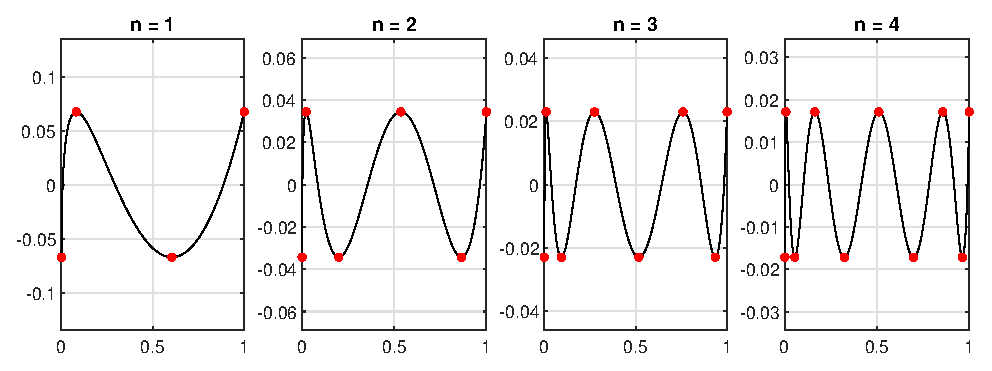
\includegraphics[width=\textwidth,height=\textheight,keepaspectratio]{figures/chapter_2/sqrtnew.eps}
    \caption{The equioscillation property demonstrated: error $E_{2n}(x)=\sqrt{x}-p^*_{2n}(x)$ in the uniform best approximations $p^*_{2n}\in\Pee_{2n}$ to $\sqrt x$ on $[0,1]$.}
    \label{fig:sqrt}
\end{figure}

In \cite[Lemma 2]{YujiZolotFreund}, Nakatsukasa and Freund provide an equioscillation result for \textit{rational} best approximations on a disjoint union of closed, bounded intervals in the uniform sense. In Theorem \ref{disjointrat}, we will generalise and prove their result to include errors equipped with a positive weight function, allowing for the same result in the relative sense, for example. We highlight the result in the case of polynomials, since it will be crucial in our construction of a composite polynomial approximation to the sign function in the next chapter.

\begin{corollary}\label{disjoint}
Suppose that $f\in C(I\cup J)$ is a real function on disjoint, closed, bounded intervals $I,J$. Then $p \in \Pee_n$ is the unique best approximation to $f$ with respect to $w$ if $(f-p)w$ equioscillates between at least $n+3$ extrema.
\end{corollary}

%\begin{proof}
%By contradiction. If $(f-r)w$ equioscillates between $n+3$ extrema %$\{x_i\}_{i=1}^{n+3}$ but there exists $p' \in \Pee_n$ such that 
%\[\norm{(f-p')w}_{\infty,I\cup J} < \norm{(f-p)w}_{\infty,I\cup J},\]
%then $(p-p')w$ takes alternating signs at the $x_i$, hence $(p-p')w$ vanishes at a minimum of $n+1$ points (this would be $n+2$ if we were not considering a disjoint union). Since $w>0$ and $p-p' \in \Pee_n$, we must have $p-p'=0$, a contradiction.
%\end{proof}

One final result on best approximations, mentioned briefly in \cite[p. 2]{Erem} as a remark, is the following. We present it as a lemma with a full proof.

\begin{lemma}\label{symm}
Let $n\in\N$, and suppose $f\in C(I)$ is an odd function on an interval $I$ symmetric about the origin. Then the best uniform approximation $p^* \in \Pee_{2n}$ is an odd function. Hence $p^*(x)=xh(x^2)$ for some $h \in \Pee_{n-1}$.
\end{lemma}

\begin{proof}
Define $q(x)=(p^*(x)-p^*(-x))/2$. Then $q(-x)=-q(-x)$, so $q$ is odd. As a result, if we write $q(x)=\sum_{k=0}^{2n} \alpha_k x^k$ for some $\alpha_k \in \R$ and compare the coefficients of the equation $q(x)=-q(-x)$, we find that $\alpha_i=0$ for $i=0,2,\dots,2n$. Hence $q(x)=\sum_{k=0}^{n-1} \alpha_{2k+1}x^{2k+1}$, so we can write $q(x)=xh(x^2)$ where 
\[h(x)=\sum_{k=0}^{n-1}\alpha_{2k+1}x^k \in \Pee_{n-1}.\]
We show that $p^*=q$. To see this, we use that $f$ is an odd function and $I$ is symmetric about the origin, so that $x \in I$ if and only if $-x \in I$, to obtain
\[ |q(x)-f(x)| = \left|\dfrac{p^*(x)-f(x)}{2}-\dfrac{p^*(-x)-f(-x)}{2}\right| \leq \norm{p^*-f}_{\infty,I},\]
by the triangle inequality. Hence $\norm{q-f}_{\infty,I} \leq \norm{p-f}_{\infty,I}$ for all $p\in\Pee_{2n}$. By uniqueness of the best approximation, we must have $p^*=q$.
\end{proof}

\textit{Remark.} In the context of Lemma \ref{symm}, the maximum uniform error of $p^*$ on $I^+=\{x \in I: x \geq 0\}$ will be identical to that on $I^-=\{x \in I: x \leq 0\}$ by symmetry, so the problem of finding the best approximation $p^*\in \Pee_{2n}$ to $f$ on $I$ is equivalent to finding the best odd approximation on $f|_{I^+}$, and such an approximation will be characterised by $f-p^*$ having at least $n+1$ equioscillation points in $I^+$. 

\subsection{Rational best approximation and equioscillation}

We occasionally discuss rational functions in this dissertation, and use the results of composite rational functions\footnote{Analogous to Definition \ref{comppolydefn}, a composite rational function is defined using bivariate rational functions, which we include in Appendix \ref{compratappendix}. This is the same definition as used in \cite{Yuji}.} as motivation for considering similar composite polynomial approximations. As such, we shall briefly discuss the analogues of this section for rational functions. 

\bigskip{}

Suppose we approximate a continuous function $f\in C(I)$ with a rational function $r_{m,n} \in \Arr_{m,n}(I)$. A \textit{rational best approximation} to $f$ with respect to a positive weight function $w$ minimises an error of the form
\[\norm{(f-r)w}_{\infty,I}\]
over all $r\in \Arr_{m,n}(I)$. A characterisation of the best approximations in terms of an equioscillating error curve also exists for rational functions \cite[Chapter II]{AkhApprox}.

\begin{thm}[Equioscillation theorem for rational functions]\label{equithmrats}
Let $f \in C(I)$ be a real function on a closed, bounded interval $I$. For every $m,n \in \N$ and weight function $w\in C(I)$, there is a unique rational best approximation $r^* \in \Arr_{m,n}$ to $f$ with respect to $w$. Moreover, if $r=P/Q$ for $P \in \Pee_m$, $Q \in \Pee_n$, then $r = r^*$ if and only if $(f-r)w$ equioscillates between at least $m+n+2-d_r$ extrema, where 
\[d_r=\min\{m-\deg P,n-\deg Q\}\]
is the \emph{defect} of $r$.
\end{thm}

Finally, we include the equioscillation result of Nakatsukasa and Freund, which we have generalised to include a weight function. This will later be used to verify the optimality of rational approximations to the sign function.

\begin{thm}\label{disjointrat}
Let $m,n \in \N$, $r \in \Arr_{m,n}$ and $f \in C(I \cup J)$, where $I,J$ are disjoint closed, bounded intervals. If $(f-r)w$ equioscillates between at least $m+n+3$ extrema, then $r$ is the (unique) rational best approximation to $f$ in $\Arr_{m,n}$ with respect to $w$.
\end{thm}

\begin{proof}
By contradiction. If $(f-r)w$ equioscillates between $m+n+3$ extrema $\{x_i\}_{i=1}^{m+n+3}$ but there exists $r' \in \Arr_{m,n}$ such that 
\[\norm{(f-r')w}_{\infty,I\cup J} < \norm{(f-r)w}_{\infty,I\cup J},\]
then $(r-r')w$ alternates in sign at the $x_i$, hence $(r-r')w$ vanishes at a minimum of $m+n+1$ points (this would be $m+n+2$ points if we were not considering a disjoint union). Since $w>0$ and $r-r' \in \Arr_{m+n,2n}$, we must have $r-r'=0$, a contradiction.
\end{proof}

\section{Matrix iterations and Newton's Method}

In the introduction, we saw how matrix iterations can be interpreted as composite polynomial or rational approximations to a matrix function $f(A)$ in terms of the initial guess $X_0$ (usually $X_0=A$). When deriving matrix iterations, it is common to first apply Newton's Method to an algebraic equation which has $f(A)$ as a solution, then choose an initial guess $X_0$ that accelerates the algorithm. Recall Newton's Method for finding a root $x^*$ of $f(x)=0$, where $f$ is a differentiable scalar function: for an initial guess $x_0$, we define the sequence
\begin{align}
    x_{k+1}=g(x_k):=x_k - \dfrac{f(x_k)}{f'(x_k)}, \qquad k=0,1,2,\dots,\label{NMeth}
\end{align}
provided that $f'(x_k)\neq 0$ for all $k$. Newton's Method converges if $x_0$ is sufficiently close to $x^*$, in this case converging quadratically \cite[Theorem 1.8]{Suli}. Due to the division by $f'(x_k)$ in \eqref{NMeth}, we often find that scalar Newton iterations contain inverses of the previous iterate. This is unfavourable if the underlying iteration function $g$ is then used to derive matrix iterations $X_{k+1}=g(X_k)$, since each iteration requires a new inverse to be computed, such as in the Newton iteration for the matrix square root \eqref{newty}.

\bigskip{}

The following example demonstrates this pitfall, and shows how considering a different algebraic equation can result in a sequence that doesn't require a new inverse to be computed at each iteration.

\begin{ex}\label{altexample}
To obtain an approximation to $\sqrt{x}$ on some interval $I$, we can fix $\lambda \in I$ and apply Newton's Method to functions for which $\sqrt{\lambda}$ is a solution. This generates iterates $x_k(\lambda)\approx \sqrt{\lambda}$ which can then be generalised to a function over the whole interval by defining $f_k(\lambda):=x_k(\lambda)$. Applying Newton's Method to the equation $f(x)=x^2-\lambda$, we obtain the iteration
\begin{align}
    f_{k+1}(x) = \dfrac{1}{2}\left(f_k(x) + \dfrac{x}{f_k(x)}\right)=:g(x,f_k(x)), \label{iter}
\end{align}
which is the scalar Newton iteration seen in \eqref{funkyiter}. Alternatively, we could apply Newton's Method to $f(x)=1-\lambda/x^2$, which also has $\sqrt{\lambda}$ as a root. This gives
\begin{align}
    f_{k+1}(x) = \dfrac{f_k(x)}{2}\left(3 -\dfrac{f_k(x)^2}{x}\right)=:\tilde{g}(x,f_k(x)). \label{altnewt}
\end{align}
\end{ex}

\begin{figure}[t!]
\centering
   \includegraphics[width=0.7\textwidth,height=0.7\textheight,keepaspectratio]{figures/chapter_2/sqrt_newton_vs_alt.eps}
   \caption{Comparison of the maximum absolute uniform error in the standard Newton \eqref{funkyiter} and Alternative Newton \eqref{altnewt} iterates to $\sqrt{x}$ on $[\delta^2,1]$, where $\delta=0.1$.}
   \label{fig:sqrt_newt_vs_alt}
\end{figure}

\begin{rmk}
While the iteration function $\tilde{g}$ in \eqref{altnewt} is not a polynomial, the iterative process never divides by the previous iterate. Furthermore, it is clear that any initial guess $f_0$ that is a multiple of $x$ will produce polynomial approximations. We will refer to the iterations \eqref{altnewt}, with $f_0(x)=x$, as \textit{Alternative Newton} iterates. 
\end{rmk}

\newpage

Figure \ref{fig:sqrt_newt_vs_alt} compares the maximum uniform error in the Newton and Alternative Newton approximations to $\sqrt{x}$. Clearly, the alternative iterates underperform the standard iterates, which is to be expected since we are comparing the convergence of polynomial approximations to rational approximations. 

\subsection{Newton-Schulz iterations and the matrix sign function}

The conventional approach for removing inverses in matrix iterations of the form $X_{k+1}=g(X_k)$, where $g$ is a rational function, is to replace all instances of $X_k^{-1}$ with inversion-free approximations to them. This can be achieved by considering Newton's Method for the inverse of an invertible matrix $B$, given by
\begin{align}
    Y_{k+1}=Y_k(2I-BY_k), \label{schulzy}
\end{align}
as proposed by Schulz \cite{schulz}. Computing one step of Newton's Method for $X_k^{-1}$ by taking $Y_k = B = X_k$ in \eqref{schulzy}, we obtain the approximation $X_k^{-1} \approx X_k(2I-X_k^2)$. Newton iterations that approximate appearances of inverses in this way are referred to as \textit{Newton-Schulz} iterations. 

\bigskip{}

Let us find the Newton-Schulz iteration for the \textit{matrix sign function}. Analogous to the scalar sign function $\sgn(z)=z/\sqrt{z^2}$, where $\text{Re}(z)\neq 0$, we define\footnote{There are several equivalent definitions for matrix functions, which are discussed in detail in \cite[Chapter 1]{Higham}.} the sign of a matrix $A \in \C^{n\times n}$ with eigenvalues away from the imaginary axis by
\[\sgn(A)=A(A^2)^{-1/2},\]
where $B^{-1/2}$ denotes the inverse of the principal square root of $B$. In particular, this is well-defined since $A$ having no eigenvalues on the imaginary axis implies that $A^2$ has no eigenvalues on the closed negative real axis. In \cite[Section 1.3]{roberts}, Roberts shows that the iteration
\begin{align}
    X_{k+1}=\dfrac{1}{2}(X_k + X_k^{-1}), \qquad X_0 = A, \label{newtonsign}
\end{align}
converges to $\sgn(A)$. The iteration is precisely Newton's Method applied to the equation $X^2=I$, for which $\sgn(A)$ is clearly a solution, hence convergence is quadratic. Replacing $X_k^{-1}$ in \eqref{newtonsign} with the approximation $X_k(2I-X_k^2)$, we obtain the Newton-Schulz iteration
\begin{align*}
    X_{k+1}=\dfrac{X_k}{2}(3I - X_k^2), \qquad X_0 = A.
\end{align*}
This sequence also converges quadratically---provided that $\norm{I-A^2}_2<1$, where $\norm{\cdot}_2$ denotes the matrix 2-norm\footnote{It can be shown that the 2-norm of a matrix $B$ is equal to $\sigma_{\max}(B)$, the largest singular value of $B$. In the case of Hermitian matrices, the singular values are equal to the absolute values of the eigenvalues (see e.g$.$ \cite{NLAbook}), hence the Newton-Schulz iterates for $A$ are quadratically convergent when the eigenvalues of $A$ have magnitude strictly less than $\sqrt{2}$. It may thus be required to scale $A$ down to a matrix with suitably small eigenvalues before proceeding.}---though many iterations are required before quadratic convergence is seen \cite[Theorem 1.1]{chen}. Similarly, in the scalar case we could approximate $\sgn(x)$ using the functions
\begin{align}
f_{k+1}(x)=g(f_k(x)), \qquad g(x)=\dfrac{x}{2}(3-x^2),\label{scalarNSsign}
\end{align}

\begin{figure}[t!]
    \centering
    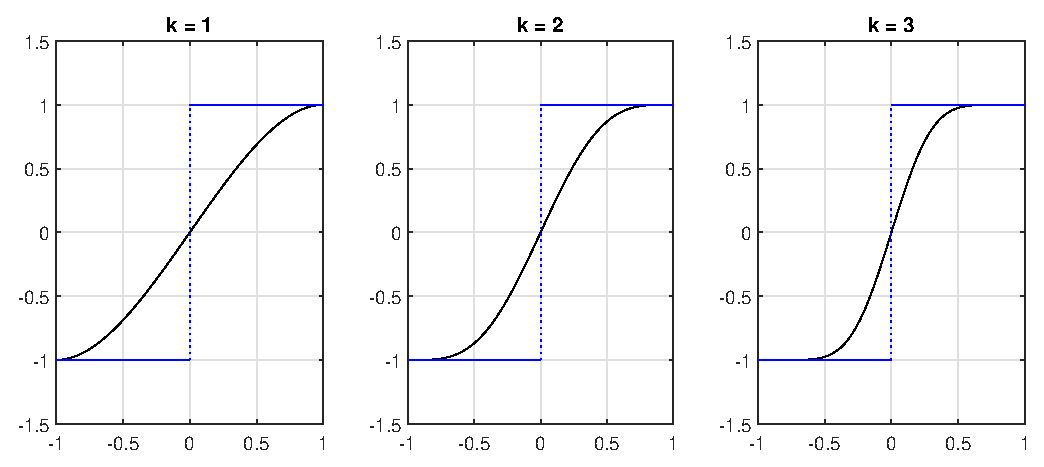
\includegraphics[width=\textwidth,height=\textheight,keepaspectratio]{figures/chapter_2/Sign_undershoot.eps}
    \caption{Newton-Schulz iterates $f_{k+1}(x)=f_k(x)(3-f_k(x)^2)/2$ (black) to $\sgn(x)$ (blue) on $[-1,1]$.}
    \label{fig:NSsigny}
\end{figure}

with $f_0(x)=x$. We shall refer to \eqref{scalarNSsign} as the \textit{(unscaled) Newton-Schulz} iteration for $\sgn(x)$. The first few iterations are illustrated in Figure \ref{fig:NSsigny}: the uniform error of the Newton-Schulz iteration is always 1 at the origin, so in practice we will consider the iteration on $X(\delta)=[-1,-\delta]\cup[\delta,1]$ for some $\delta \in(0,1)$. The maximum uniform error is then given by
\[\norm{f_k-\sgn}_{\infty,X(\delta)}=f_k(\delta).\]
\begin{rmk}
The Newton-Schulz iteration is one of a family of iterations of the form $X_{k+1}=g_{m,n}(X_k)$, where $g_{m,n}(x)=x p_m(1-x^2)/q_n(1-x^2)$, used for computing $\sgn(A)$. Here $p_m/q_n$ represents the $[m/n]$ \textit{Padé approximant} of $(1-x)^{-1/2}$ (see e.g. \cite[Section 3]{kenneylaubrational}). When $n=0$, we obtain composite polynomial approximations; in particular we recover the Newton-Schulz iteration for $(m,n)=(1,0)$. 
\end{rmk} 

%\subsection{Iterations for the square root function} 

%The result of Higham, Mackey, Mackey, and Tisseur states that, when $A^{1/2}$ is well-defined, any iteration $X_{k+1}=X_k h(X_k^2)$ converging to $\sgn\left(\begin{bsmallmatrix} 0 & A \\ I & 0 \end{bsmallmatrix}\right)$ gives rise to a coupled iteration 
%\[\begin{cases}Y_{k+1}=Y_k h(Z_k Y_k), & \quad Y_0 = A, \\ Z_{k+1} = h(Z_kY_k)Z_k, & \quad Z_0=I,\end{cases}\]
%in which $Y_k \to A^{1/2}$ and $Z_k \to A^{-1/2}$ as $k\to\infty$, with the same order of convergence as the $X_k$ \cite[Theorem 6.11]{Higham}. Taking $h(X)=(3I-X)/2$, the iteration function for the Newton-Schulz iterates to the sign function, we obtain
%\[\begin{cases}Y_{k+1}=Y_k (3I-Z_kY_k)/2, & \quad Y_0 = A, \\ Z_{k+1} = (3I-Z_kY_k)Z_k/2, & \quad Z_0=I,\end{cases}\]
%a coupled Newton-Schulz iteration for approximating the principal square root %$A^{1/2}$ and its inverse. Similarly we use the coupled scalar functions
%\begin{align}
%    \begin{cases}f_{k+1}(x)=f_k(x) (3-g_k(x)f_k(x))/2, & \quad f_0(x) = x, \\ g_{k+1}(x) = g_k(x)(3-g_k(x)f_k(x))/2, & \quad g_0(x)=1,\end{cases} \label{scalarNSsqrt}
%\end{align}
%to approximate $\sqrt{x}$ and $1/\sqrt{x}$ respectively. Figure \ref{fig:sqrterrors} sketches the error in the $f_k$ for the first 6 iterations.

%\begin{figure}[t!]
%    \centering
%    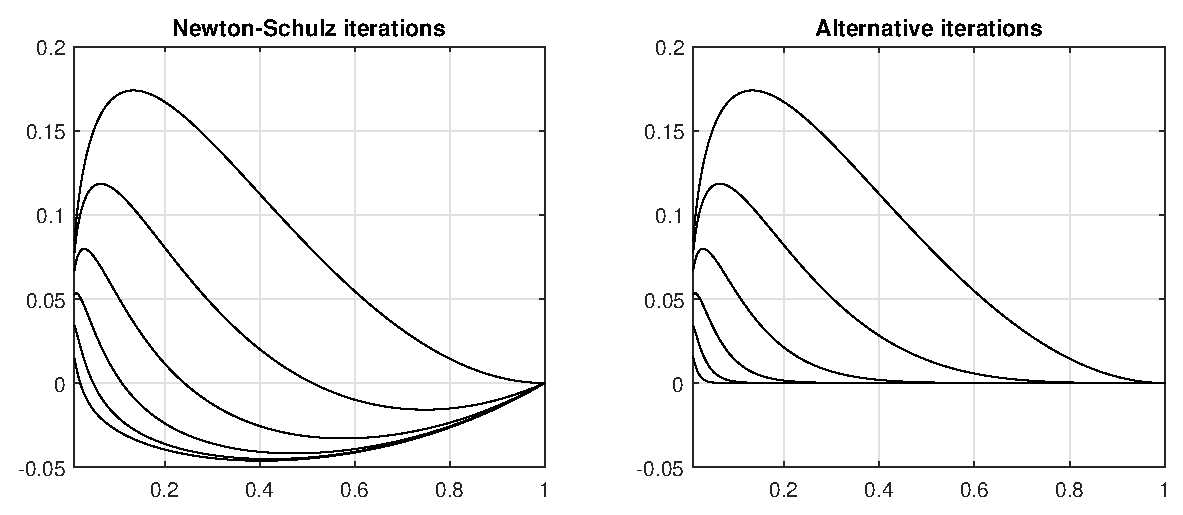
\includegraphics[width=\textwidth,height=\textheight,keepaspectratio]{sqrt_NSvsalt.eps}
%    \caption{Error $E_k(x)=\sqrt{x}-f_k(x)$ in the Newton-Schulz \eqref{scalarNSsqrt} and alternative \eqref{alt} iterations $f_k$ to $\sqrt{x}$ on $[0.1^2,1]$, for $k=1,\dots,6$.}
%    \label{fig:sqrterrors}
%\end{figure}





%One of the earliest methods of approximating the square root, \textit{Heron's Method}, dates back to the first century. For $\lambda>0$, Heron's Method for approximating $\sqrt{\lambda}$ is given by the following iterative process. Let $x_0$ be an initial guess. Then either $x_0$ or $\lambda/x_0$ is greater than $\sqrt{\lambda}$, whilst the other quantity is less than $\sqrt{\lambda}$. Let $x_1$ be the average of these two quantities. Repeat this averaging process with the new guess, and so forth. We can write this as $x_{k+1}=(x_k + \lambda x_k^{-1})/2$, where $k\in \N$. This process is equivalent to applying Newton's Method to solve the equation $x^2-\lambda=0$.

%Adopting the notation used in Appendix \ref{improvenewton}, the improved method is defined by $F_0(x)=C_0 f_0(x)$ and
%\begin{align}
%    F_{k+1}(x) = \dfrac{C_{k+1}}{2}\left(F_k(x)+\dfrac{x}{F_k(x)}\right),
%\end{align}
%where the constants $C_k$ are defined by
%\[C_0 = \dfrac{1}{\sqrt{s'_0 s''_0}}, \qquad C_k = %\dfrac{1}{\sqrt{N^*(S''_{k-1})}} \qquad (k\geq 1),\]
%and $S''_k=\max_{x\in I} F_k(x)/\sqrt x$.



%Alternatively we could approximate $\sqrt{\lambda}$ by first approximating $1/\sqrt{\lambda}$ with iterates $x_k$, then noting that $\sqrt{\lambda} \approx \lambda x_k$.

%\begin{ex}
%Suppose for $\lambda >0$ we want to approximate the value of $1/\sqrt{\lambda}$. This is equivalent to finding the positive root of $f(x)=x^2-1/\lambda=0$, so Newton's Method reads
%\[x_{k+1} = x_k - \dfrac{x_k^2-1/\lambda}{2x_k} = \dfrac{1}{2}\left(x_k +\dfrac{1}{\lambda x_k}\right).\]
%Alternatively, if we solved for the root of $f(x)=1/x^2-\lambda$, we obtain
%\begin{align}
 %   x_{k+1} = x_k - \dfrac{1/x_k^2-\lambda}{-2/x_k^3} = \dfrac{x_k}{2}\left(3 -\lambda x_k^2\right). \label{NEWTON2}
%\end{align}
%We similarly note that \eqref{NEWTON2} never divides by the previous iterate.
%\end{ex}


\subsection{Improved Newton's Method}\label{improvednewtonsection}

Despite being a quadratically converging sequence, the Newton-Schulz iteration \eqref{scalarNSsign} can take a large number of iterations to reach a suitably small error. For example, when $\delta=10^{-2}$, it takes 14 iterations to obtain an error $\ep<10^{-2}$ on $X(\delta)$. This is because the order of convergence is an \textit{asymptotic} property, and in practice, convergence breaks down into two phases:
\begin{itemize}
    \item the number of iterations required to reduce the error to some small value;
    \item the asymptotic behaviour given by the order of convergence.
\end{itemize}
Crucially, this means that we cannot guarantee that a quadratically convergent sequence (such as Newton's Method, or the Newton-Schulz iterates) will converge in a small number of iterations. 

\bigskip{}

Many contributions have been made to reduce the number of iterations required in the initial phase of convergence by considering scaled iterative processes, such as in \cite{ninomiya1970best,Rutishauser}. These processes generally take the form $f_{k+1}(x)=g_{k+1}(x,f_k(x))$, where the iteration functions $g_k$ suitably scale each new iteration based on the previous one. For example, Ninomiya provides an improved version of Newton's Method for $\sqrt{x}$ on $I=[a,b]$ where $0<a<b$ in \cite{ninomiya1970best}, after noting that each iteration of \eqref{iter} has an upward bias. In this subsection, we will show how he proved this observation, and discuss the scaled iteration he proposed. We begin by defining
\[N^*(x)=\dfrac{1}{2}(x+x^{-1}), \qquad x>0,\]
and observe the following properties:
\begin{enumerate}
    \item[(1)] $N^*(x) \geq N^*(1) = 1$;
    \item[(2)] $xy=1 \Longrightarrow N^*(x)=N^*(y)$;
    \item[(3)] $(xy-1)(x-y)>0 \Longleftrightarrow N^*(x)>N^*(y)$.
\end{enumerate}
With the $f_k$ as in \eqref{iter}, we can write
\[s_{k+1}(x) = N^*(s_k(x)), \qquad s_k(x)=\dfrac{f_k(x)}{\sqrt{x}}.\]
Writing the Newton iterates in this way, and defining
\[s'_k=\min_{x\in I} s_k(x), \qquad s''_k=\max_{x\in I} s_k(x),\]
we see that $s'_k = \min_{x\in I} N^*(s_{k-1}(x)) \geq 1$ for $k=1,2,\dots$, from condition (1). Moreover, by condition (3) we have
\begin{align}
    s'_k s''_k >1. \label{overest}
\end{align}

\begin{figure}[t!]
\centering
   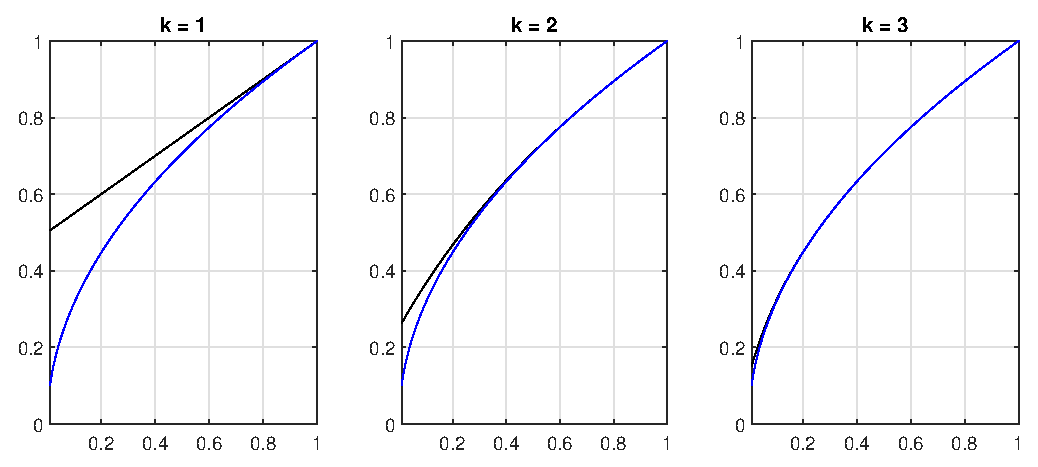
\includegraphics[width=\textwidth,height=\textheight,keepaspectratio]{figures/chapter_2/Newton_overshoot.eps}
   \caption{Newton iterates $f_{k+1}(x)=(f_k(x)+x/f_k(x))/2$ (black), plotted with $\sqrt{x}$ (blue) on $[\delta^2,1]$, where $\delta=0.1$. The $f_k$ always overestimate $f$ in the sense of \eqref{overest}.}
   \label{fig:overshootnewton}
\end{figure}

Figure \ref{fig:overshootnewton} demonstrates this effect, which is problematic because it means that the error in iterations can never equioscillate, for instance. With the aim of finding a sequence that satisfies $s'_ks''_k=1$, Ninomiya proposes the improved Newton iterates
\begin{align}
   F_{k+1}(x) = \dfrac{C_{k+1}}{2}\left(F_k(x)+\dfrac{x}{F_k(x)}\right), \qquad k=0,1,2,\dots, \label{improvnewty}
\end{align}
with $F_0=f_0/\sqrt{s'_0s''_0}$. The constants $C_{k+1}$ are given by
\[C_{k+1} = \dfrac{1}{\sqrt{N^*(S''_{k})}}, \qquad S''_k = \max_{x\in I} \dfrac{F_k(x)}{\sqrt{x}}.\]

\begin{figure}[t!]
\centering
   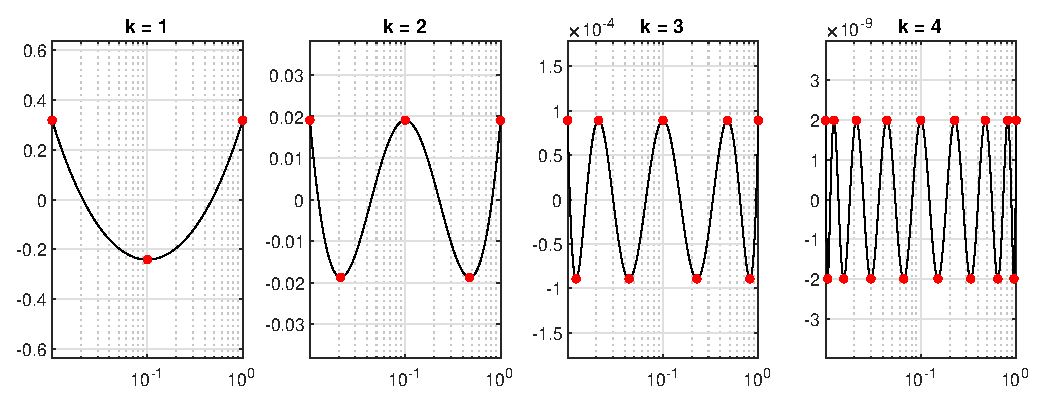
\includegraphics[width=\textwidth,height=\textheight,keepaspectratio]{figures/chapter_2/improvednewton_rational.eps}
    \caption{Relative error $E_k(x)=F_k(x)/\sqrt{x}-1$ in Ninomiya's improved Newton iterates \eqref{improvnewty} to $\sqrt{x}$ on $[\delta^2,1]$, where $\delta=0.1$.}
   \label{fig:improvednewton_rational}
\end{figure}

Assuming that we have optimised our initial guess so that $s'_0s''_0=1$, Ninomiya analyses the convergence of the $F_k$ using the following recursions, whose proofs were omitted from his paper. We prove them here as a technical lemma.

\begin{lemma}\label{EEEk}
The maximum relative errors $e''_k=s''_k-1$ and $E''_k=S''_k-1$ satisfy
\[e''_{k+1}=\dfrac{{e''_k}^2}{2(1+e''_k)}, \qquad E''_{k+1}=\sqrt{\dfrac{{E''_k}^2}{2(1+E''_k)}+1}-1.\]
\end{lemma}

\begin{proof}
Let $e_k(x)=s_k(x)-1$ and $E_k(x)=S_k(x)-1$ be the relative errors of $f_k(x)$, $F_k(x)$ respectively. Then
\begin{align*}
    e_{k+1}(x) &= s_{k+1}(x)-1 \\
    & = \dfrac{1}{2}\left(s_k(x)+\dfrac{1}{s_k(x)}\right) -1\\
    & = \dfrac{1}{2}\left(e_k(x)+1+\dfrac{1}{e_k(x)+1}\right) -1\\
    &=\dfrac{e_k(x)^2}{2(1+e_k(x))}.
\end{align*}
Since $x \mapsto x^2(1+x)^{-1}$ is an increasing function on $[0,1]$, $e_{k+1}(x)$ obtains its maximum when $e_k(x)$ is maximised, i.e. $e''_{k+1}={e''_k}^2/(2(1+e''_k))$. Similarly we have
\begin{align*}
    E_{k+1}(x) & =S_{k+1}-1 \\
    &=\dfrac{C_{k+1}}{2}\left(S_k(x)+\dfrac{1}{S_k(x)}\right) -1 \\
    &=\dfrac{1}{2\sqrt{N^*(E''_k+1)}}\left(E_k(x)+1+\dfrac{1}{E_k(x)+1}\right) -1 \\
    &=\dfrac{1}{\sqrt{N^*(E''_k+1)}}\left(\dfrac{E_k(x)^2}{2(1+E_k(x))}+1\right)-1.
\end{align*}
As before, $E_{k+1}(x)$ obtains its maximum when $E_k(x)$ is maximised, giving
\begin{align*}
    E''_{k+1}&=\dfrac{1}{\sqrt{N^*(E''_k+1)}}\left(\dfrac{{E''_k}^2}{2(1+E''_k)}+1\right)-1 \\
    &= \sqrt{\dfrac{{E''_k}^2}{2(1+E''_k)}+1}-1,
\end{align*}
by definition of $N^*$, as required.
\end{proof}

By Lemma \ref{EEEk} and a Taylor expansion, we obtain the approximate relations
\[e''_{k+1} \sim \dfrac{{e''_k}^2}{2}, \qquad E''_{k+1} \sim \dfrac{{E''_k}^2}{4}\]
as $k\to\infty$. Combining with $E''_0=e''_0$, we obtain the approximate relation
\[E''_k \sim \dfrac{e''_k}{2^{2^k-1}},\]
demonstrating that the iterates \eqref{improvnewty} improve convergence. Figure \ref{fig:improvednewton_rational} sketches the relative error of the improved Newton iterates \eqref{improvnewty}, which appear to be the best rational approximants in the relative sense as they have the correct number of equioscillation points\footnote{To see this, we note that $F_k$ is of type $(2^{k-1},2^{k-1}-1)$ by induction, hence the best rational approximant equioscillates between at least $2^k+1-d_{F_k}$ extrema by Theorem \ref{equithmrats}.}. However, they do not equioscillate between $\pm E''_k$ upon closer inspection. Ninomiya shows that the $F_k$ are best approximations over all $R$ of the same order with respect to the error of $g(x,R(x))$ relative to $\sqrt{x}$, where $g$ is the standard Newton iteration \eqref{iter} for $\sqrt{x}$ (see \cite[Theorem 4]{ninomiya1970best} for details). 

\bigskip{}

While Ninomiya's improved Newton iteration \eqref{improvnewty} is not a composite polynomial approximation to $\sqrt{x}$, we can consider his work as motivation for constructing such an approximation. Ideally, the error of our approximation should not display an upward bias, and have a similar error curve to that of Figure \ref{fig:improvednewton_rational}. In general, this dissertation is concerned with constructing polynomial approximations, such as to the Newton-Schulz approximation \eqref{scalarNSsign} to $\sgn(x)$ and the Alternative Newton approximation \eqref{altnewt} to $\sqrt{x}$, for which the convergence is accelerated. From the discussion of this section, it seems reasonable that suitably scaling the existing methods at each iteration is a sure-fire way to proceed. In the next chapter, we take a different approach to constructing an approximation to the sign function, yet discover that our method is in fact equivalent to a scaled Newton-Schulz method.

%\subsection{Halley's Method}

%An advance on Newton's Method for rootfinding is due to Halley, who developed an algorithm which finds approximations to $C^2$ functions with a cubic convergence rate. The derivation is as follows: consider a function $f$ with unknown root $x^*$, and its second-order Taylor approximation
%\[f(x) \approx f(x_k) + f'(x_k)(x-x_k) + \dfrac{f''(x_k)}{2}(x-x_k)^2,\]
%where $x_k$ is an approximate root of $f$. In a similar way to Newton's Method, we use the Taylor approximation to determine a point $x_{k+1}$ that better approximates $x^*$ than $x_k$. For this we solve
%\[f(x_k) + f'(x_k)(x_{k+1}-x_k) + \dfrac{f''(x_k)}{2}(x_{k+1}-x_k)^2 = 0,\]
%which can be factorised and re-arranged to obtain
%\[x_{k+1}-x_k= \dfrac{-f(x_k)}{f'(x_k)+\frac{f''(x_k)}{2}(x_{k+1}-x_k)}.\]
%By replacing $x_{k+1}-x_k$ on the right hand side with the error between consecutive iterates in Newton's Method, i.e. $x_{k+1}-x_k = -f(x_k)/f'(x_k)$, we obtain
%\begin{align}
%    x_{k+1} = x_k -\dfrac{2f(x_k)f'(x_k)}{2f'(x_k)^2-f(x_k)f''(x_k)}.\label{halley}
%\end{align}
%The iterative procedure \eqref{halley} is known as Halley's Method.

%\bigskip{}

%\begin{ex}
%Suppose for some $\lambda >0$ we want to approximate the value of $1/\sqrt{\lambda}$. This is equivalent to finding the positive root of $f(x)=1/x^2 -\lambda=0$. Then \eqref{halley} reads
%\begin{align}
%    x_{k+1} = \dfrac{x_k}{8}\left(15-\lambda x_k^2(10-3\lambda x_k^2)\right).\label{halleyrecip}
%\end{align}
%\end{ex}



%\newpage
%\thispagestyle{empty}
%\mbox{}
% CHAPTER
\chapter{Composite polynomial approximation to \texorpdfstring{$\sgn (x)$}{sgn(x)}}\label{sgnchapter}

\section{Zolotarev functions}

To motivate the work of this chapter, we first discuss a notable result in rational approximation theory, concerning the rational best approximations to $\sgn(x)$ on 
\[X(\delta)=[-1,-\delta]\cup [\delta,1],\] 
for some $\delta \in (0,1)$. Such approximations are referred to as the \textit{Zolotarev functions}; in particular, we write $Z_{2r+1}(x;\delta)$ for type $(2r+1,2r)$ approximations. The explicit form of $Z_{2r+1}(\cdot;\delta)$ was found by Zolotarev \cite{Zolo} in terms of Jacobi elliptic functions
\[\text{sn}(u;\delta)=\sin \phi, \qquad \text{cn}(u;\delta)=\cos \phi;\]
here $\phi$ denotes the Jacobi amplitude, obtained from the inversion of the \textit{incomplete elliptic integral of the first kind} (see e.g. \cite[Chapter 5]{akhiezer})
\[u=F(\phi;\delta):=\int_0^\phi \dfrac{d\theta}{\sqrt{1-\delta^2\sin^2 \theta}}.\]
The Zolotarev functions are then given by
\begin{align}
    Z_{2r+1}(x;\delta)=Mx\prod_{i=1}^r \dfrac{x^2+c_{2i}}{x^2+c_{2i-1}}, \label{zolotarevfn}
\end{align}

\begin{figure}[t!]
\centering
   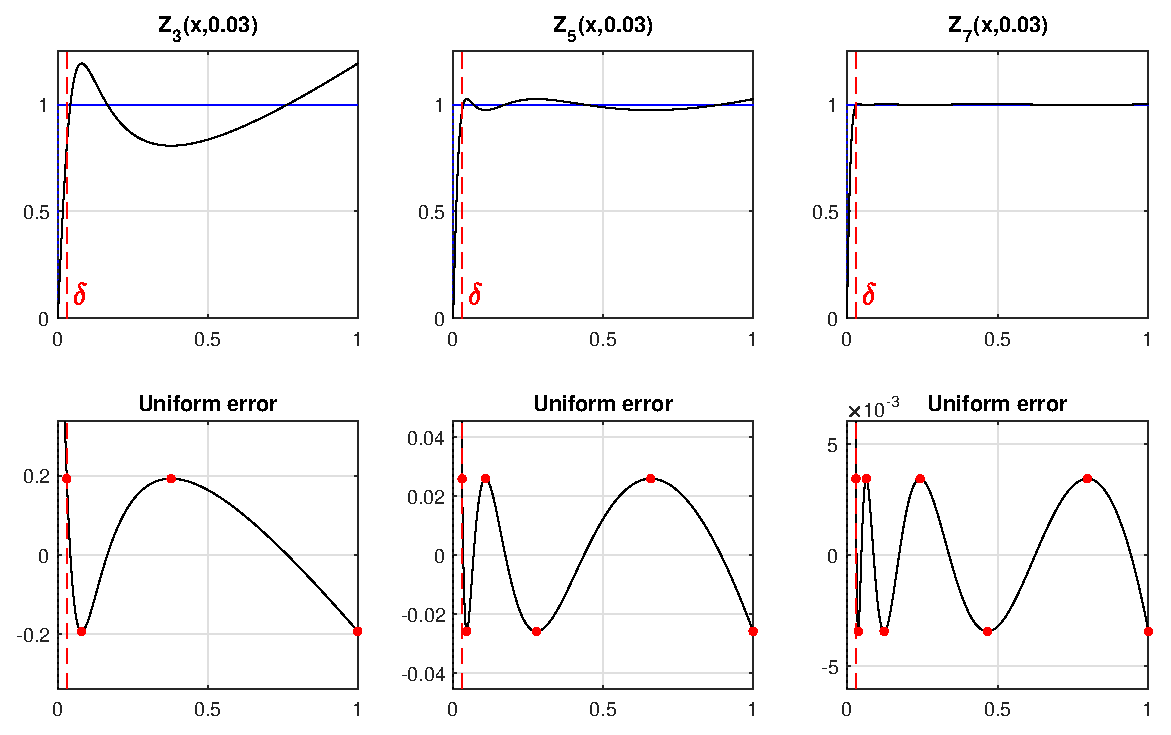
\includegraphics[width=\textwidth,height=\textheight,keepaspectratio]{figures/chapter_3/ZOLOTAREV.eps}
   \caption{Zolotarev functions $Z_{2r+1}(x;\delta)$ for $\delta=0.03$, constructed using \texttt{ellipke} and \texttt{ellipj}. The corresponding uniform error $\sgn(x)-Z_{2r+1}(x;\delta)$ is sketched below each plot, which equioscillates between $4r+4$ extrema in each case.}
   \label{fig:ZOLOT}
\end{figure}

where for $i=1,\dots,2r$ the constants $c_i$ are defined by
\[c_i=\delta^2 \dfrac{\text{sn}^2\left(\frac{iK'}{2r+1};\delta'\right)}{\text{cn}^2\left(\frac{iK'}{2r+1};\delta'\right)},\]
with $\delta'=\sqrt{1-\delta^2}$ and $K'=F(\pi/2;\delta')$ respectively denoting the \textit{complementary modulus} and \textit{complete elliptic integral of the first kind} for $\delta'$. Here, $M>0$ is a scalar determined by the equioscillation property of the best approximation, which ensures that $1-Z_{2r+1}(\delta;\delta)=-(1-Z_{2r+1}(1;\delta))$. Hence
\[M=2\left(\prod_{i=1}^r\dfrac{1+c_{2i}}{1+c_{2i-1}}+\delta \prod_{i=1}^r\dfrac{\delta^2+c_{2i}}{\delta^2 +c_{2i-1}}\right)^{-1}.\]

Nakatsukasa and Freund showed that normalised Zolotarev functions $\hat{Z}_{2r+1}(\cdot;\delta)$, which take the form \eqref{zolotarevfn} multiplied by $1/Z_{2r+1}(1;\delta)$, satisfy a recursive optimality property. Explicitly, we can write
\[\hat{Z}_{2r'+1}(\hat{Z}_{2r+1}(x;\delta_1);\delta_2) = \hat{Z}_{(2r+1)(2r'+1)}(x;\delta_1),\]
where $\delta_2$ is such that $X(\delta_2)=\hat{Z}_{2r+1}(X(\delta_1);\delta_1)$ \cite[Theorem 3]{YujiZolotFreund}. The proof involves counting equioscillation points and invoking the minimax equioscillation property. We use this as motivation for constructing a composite polynomial approximation consisting of the composition of low-order best approximations to the sign function.

\section{Greedy approximation to \texorpdfstring{$\sgn(x)$}{sgn x} in \texorpdfstring{$\Pee_{(k,3)}^{\text{comp}}$}{P k,3 comp}}

In this section, we construct a pure composite polynomial approximation to $\sgn(x)$ on $X(\delta)$ using a greedy iterative process, namely an approximation of the form
\[f_{k+1}(x) = g_{k+1}(f_{k}(x)), \qquad k=1,2,\dots,\]
where each $g_{k+1} \in \Pee_3$ is the best approximation to $\sgn(x)$ on its domain $f_{k}(X(\delta))$. We start by finding the best polynomial approximant $p \in \Pee_3$ to $\sgn(x)$ on $X(\delta)$, which is an odd function by Lemma \ref{symm}, hence has the form
\[p(x)=x(A+Bx^2),\]
for some constants $A,B$ to be determined. For simplicity, we normalise $p$ such that $\norm{p}_{\infty,X(\delta)}=1$, and as such approximate a scaled version of the sign function $C\sgn(x)$, for some constant $C \in (0,1)$ determined by the normalisation of $p$. By Corollary \ref{disjoint}, we know that $C\sgn -p$ equioscillates between at least 6 extrema: to obtain equioscillation, we can impose
\begin{align}
    p(\delta)=p(1)=2C-1, \label{valueofC}
\end{align}
so that the maximum error $1-C$ is obtained at the points  $\pm 1, \pm \delta$, $\pm \xi$, where $\xi \in (\delta,1)$ is the extremal point such that $p(\xi)=1$. This gives us three conditions:

\begin{itemize}
    \item\makebox[2cm]{$p(\delta)=p(1)$\hfill} $\quad\Longrightarrow \quad (1-\delta)A+(1-\delta^3)B=0$;
    \item\makebox[2cm]{$p'(\xi)=0$\hfill} $\quad\Longrightarrow \quad A+3\xi^2B=0$;
    \item\makebox[2cm]{$p(\xi)=1$\hfill} $\quad\Longrightarrow \quad \xi A + \xi^3 B-1=0$.
\end{itemize}

Solving these equations, we find that the best approximation is
\begin{align}
     p(x)=\dfrac{x}{2\xi}\left(3-\dfrac{x^2}{\xi^2}\right), \qquad \xi=\sqrt{\dfrac{1+\delta+\delta^2}{3}},\label{xis}
\end{align}

\begin{figure}[t!]
\centering
   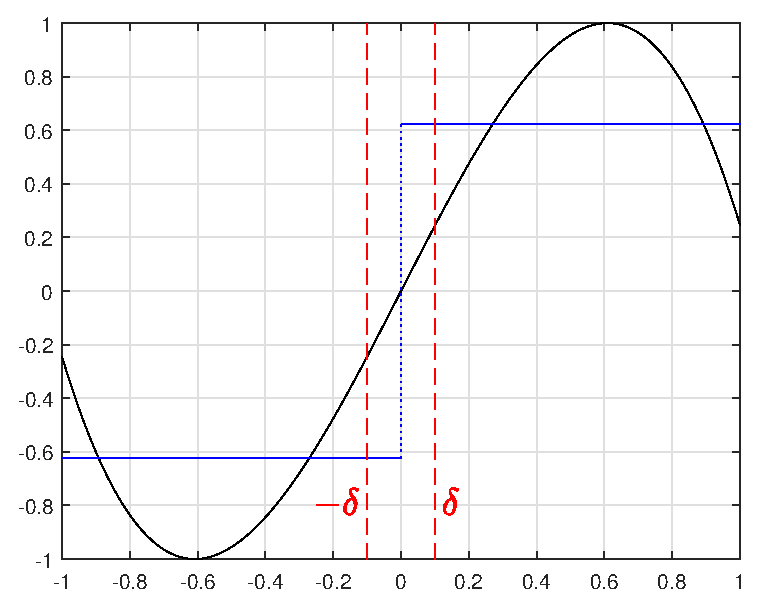
\includegraphics[width=0.6\textwidth,height=0.6\textheight,keepaspectratio]{figures/chapter_3/COMPSIGNsingle.eps}
   \caption{Best $\Pee_3$-approximation (black) to $C\sgn(x)$ (blue) on $X(\delta)$, where $\delta=0.1$.}
   \label{fig:compsign}
\end{figure}

By the symmetry of our construction, and using that $C=(1+p(\delta))/2$ by \eqref{valueofC}, we can obtain the maximum error $E$ in the approximation
\[E=1-C=\dfrac{1-p(\delta)}{2}.\]
Figure \ref{fig:compsign} sketches the approximation for $\delta=0.1$, for which the normalisation of $p$ gives $C\approx 0.6222$ and $E\approx 0.3778$.

\bigskip{}

\begin{rmk}
By symmetry, the range of $p$ is $X(p(\delta))$. In particular, the containment $X(p(\delta)) \subset X(\delta)$ is strict, thanks to the following lemma.
\end{rmk}

\begin{lemma}\label{tekky}
Given $\delta \in (0,1)$ and $p \in \Pee_3$ defined by \eqref{xis}, we have $p(\delta)>\delta$.
\end{lemma}

\begin{sproof}
There holds
\begin{align*}
    \dfrac{p(\delta)}{\delta} =\dfrac{1}{2\xi}\left(3-\dfrac{\delta^2}{\xi^2}\right)= \dfrac{3\sqrt{3}}{2}\left(\dfrac{1+\delta}{(1+\delta+\delta^2)^{3/2}}\right),
\end{align*}
so it remains to show that
\[\dfrac{3\sqrt{3}}{2}>\dfrac{(1+\delta+\delta^2)^{3/2}}{1+\delta}=:h(\delta).\]
But $h$ is strictly increasing, therefore $h(\delta)<h(1)=3\sqrt{3}/2$.
\end{sproof}

Fixing $p$ as in \eqref{xis}, we can similarly find the polynomial 
\[q \in \{f \in \Pee_3 : \norm{f}_{\infty,p(X(\delta))}=1\}\]
such that $q(p(x))$ is an optimal approximation for $D\sgn(x)$, for some scale factor $D$ determined by the normalisation of $q$. To see this, note that by the above remark, the domain of $q$ is $p(X(\delta))=X(p(\delta))$. Hence $q$ is obtained in the same manner as $p$, except with $\delta$ replaced by $p(\delta)$. Repeating this process, we obtain a sequence
\[f_{k+1}(x)=g_{k+1}(f_{k}(x)), \qquad k=0,1,2,\dots,\]
where $f_0(x)=x$ and
\begin{align}
    g_{k+1}(x) =\dfrac{x}{2\xi_{k+1}}\left(3-\dfrac{x^2}{\xi_{k+1}^2}\right), \qquad \xi_{k+1}=\sqrt{\dfrac{1+f_{k}(\delta)+f_{k}(\delta)^2}{3}}. \label{compconsts}
\end{align}

\begin{figure}[t!]
\centering
   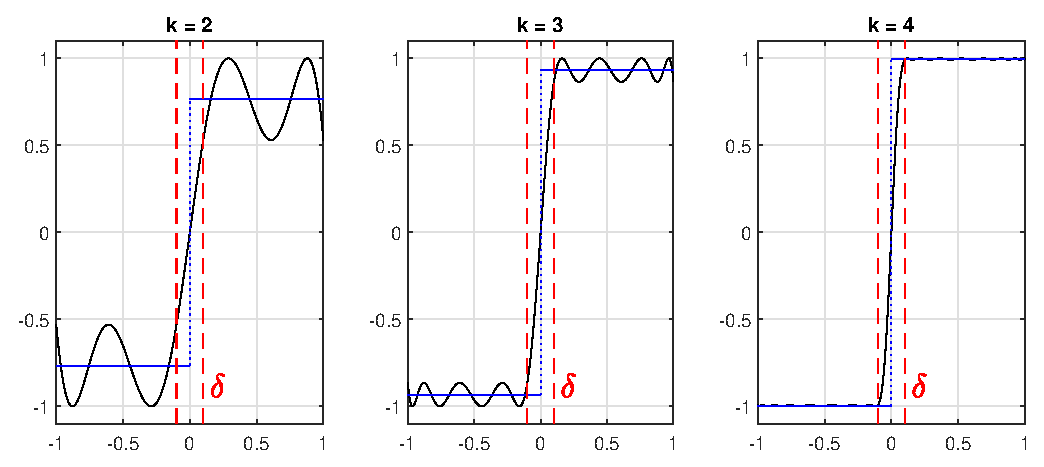
\includegraphics[width=\textwidth,height=\textheight,keepaspectratio]{figures/chapter_3/COMPSIGNthree.eps}
   \caption{Scaled Newton-Schulz iterates $f_k(x)$ (blue) with $C_k\sgn(x)$ (black) on $X(\delta)$, where $\delta=0.1$. The iterate for $k=1$ is shown in Figure \ref{fig:compsign}.}
   \label{fig:compsign2}
\end{figure}

By induction, it follows that $f_k \in \Pee_{(k,3)}^{\text{comp}}$, and is an approximation for $C_k \sgn(x)$ with maximum uniform error $E_k$, where 
\begin{align}
    C_k = \dfrac{1+f_k(\delta)}{2}, \qquad E_k = \dfrac{1-f_k(\delta)}{2}. \label{Ceekay}
\end{align}

\begin{rmk}
We note that $g_k(x) = g(x/\xi_k)$, where $g$ is the iteration function for the unscaled Newton-Schulz  approximation to the sign function \eqref{scalarNSsign}. Hence the iteration \eqref{compconsts} is equivalent to a scaled version of the of \eqref{scalarNSsign}, with $x$ replaced by $x/\xi_k$ at the $k^{\text{th}}$ iteration. As such, we will refer to \eqref{compconsts} as \textit{scaled Newton-Schulz} iterates to the sign function.
\end{rmk}

\section{Equioscillation behaviour}\label{equiSNS}

Since the scaled Newton-Schulz iterate $f_k$ has degree $3^k$, it follows by Corollary \ref{disjoint} that it is the best $\Pee_{3^k}$-approximation if $f_k-C_kf$ equioscillates between at least $3^k+3$ extrema on $X(\delta)$. By symmetry, this is the case when $f_k-C_k$ equioscillates between $(3^k+3)/2$ extrema on $[\delta,1]$. In the following technical lemma, we show that $f_k-C_k$ falls short of this number of equioscillation points.

\begin{figure}[t!]
\centering
   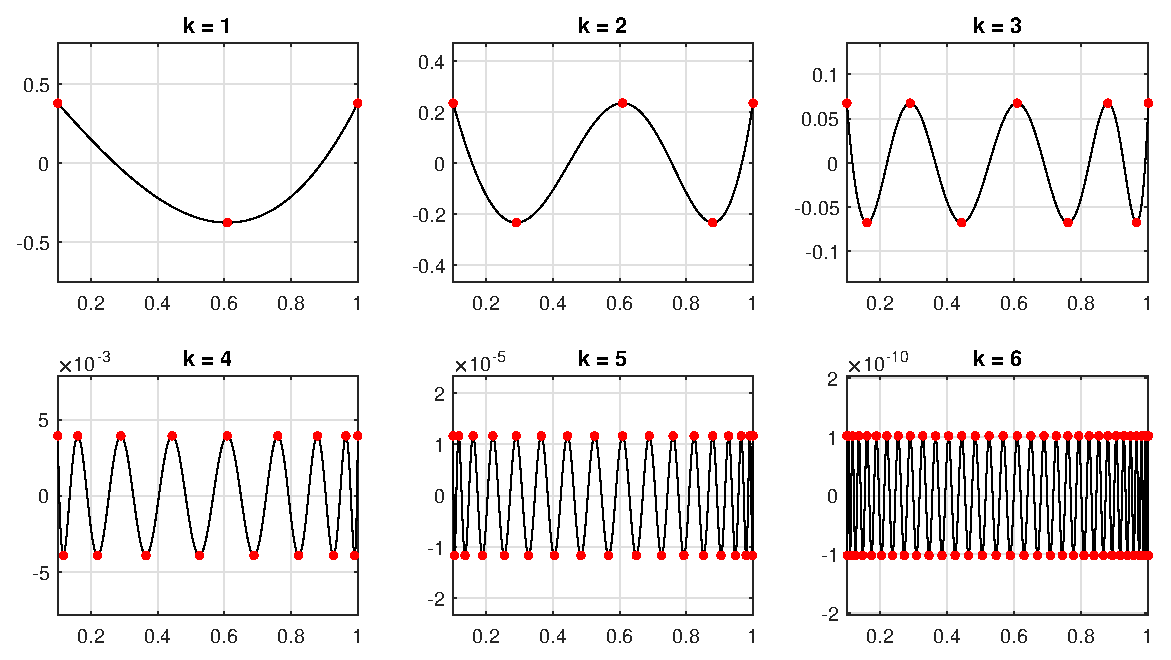
\includegraphics[width=\textwidth,height=\textheight,keepaspectratio]{figures/chapter_3/COMPSIGNMANYITERATES2.eps}
   \caption{Error $E_k(x)=C_k\sgn(x)-f_k(x)$ on $[\delta,1]$, where $\delta=0.1$. The error curve equioscillates between $2^{k}+1$ extrema in each case, as shown in Lemma \ref{equio}.}
   \label{fig:compsignmanyiterates}
\end{figure}

\begin{lemma}\label{equio}
Let $\delta \in (0,1)$ and $f_k \in \Pee_{(k,3)}^{\emph{comp}}$ be defined by \eqref{compconsts}. Then the error curve $f_k-C_k\emph{\sgn}$ equioscillates between $2^{k+1}+2$ extrema on $X(\delta)$, or equivalently, $f_k-C_k$ equioscillates between $2^{k}+1$ extrema on $[\delta,1]$.
\end{lemma}

\begin{proof}
By induction. The case for $k=1$ is clear, as we constructed $f_1$ to have 6 equioscillation points on $X(\delta)$. 

\bigskip{}

Now assume that $f_k-C_k \sgn$ equioscillates between $2^{k+1}+2$ extrema on $X(\delta)$, or equivalently between $2^k+1$ points $\{x_j\}_{j=1}^{2^k+1}$ on $[\delta,1]$. Then there are $2^k$ intervals $I_j=[x_j,x_{j+1}]$, $j=1,\dots,2^k$ such that $f_k(I_j)=[f_k(\delta),1]$.

\bigskip{}

Consider $g_{k+1}(x)$ on $[f_k(\delta),1]$. By construction, $g_{k+1}$ equioscillates between three points on this interval, namely $f_k(\delta)$, $\xi_{k+1}$ and $1$. Hence $g_{k+1}(f_k(x))$ equioscillates between 3 points on each $I_j$. Since we have $2^k$ such intervals, and $2^k-1$ points $\{x_j\}_{j=2}^{2^k}$ where equioscillation points overlap, the total number of equioscillation points of $g_{k+1}(f_k(x))$ on $[\delta,1]$ is
\[3(2^k) - (2^k-1)=2^{k+1}+1,\]
hence $2^{k+2}+2$ points on $X(\delta)$ by symmetry. But $g_{k+1}(f_k(x))=f_{k+1}(x)$, so this completes the inductive step of the theorem.
\end{proof}

\section{Convergence analysis of the scaled Newton-Schulz iterates}

We know from Section \ref{equiSNS} that the recursive optimality property of the Zolotarev functions \eqref{zolotarevfn} does not hold in the polynomial setting: composing normalised best cubic approximations to the sign function on $X(\delta)$ does not result in best approximations of higher order. However, we shall compare the convergence of the scaled Newton-Schulz iterates to the unscaled iterates and the minimax. In what follows, it will be useful to write $\delta_k:=f_k(\delta)$, so that \eqref{compconsts} reads
\begin{align}
    f_{k+1}(x) =\dfrac{f_k(x)}{2\xi_{k+1}}\left(3-\dfrac{f_k(x)^2}{\xi_{k+1}^2}\right), \qquad \xi_{k+1}=\sqrt{\dfrac{1+\delta_k+\delta_k^2}{3}}. \label{deltak}
\end{align}

\begin{figure}[t!]
\centering
   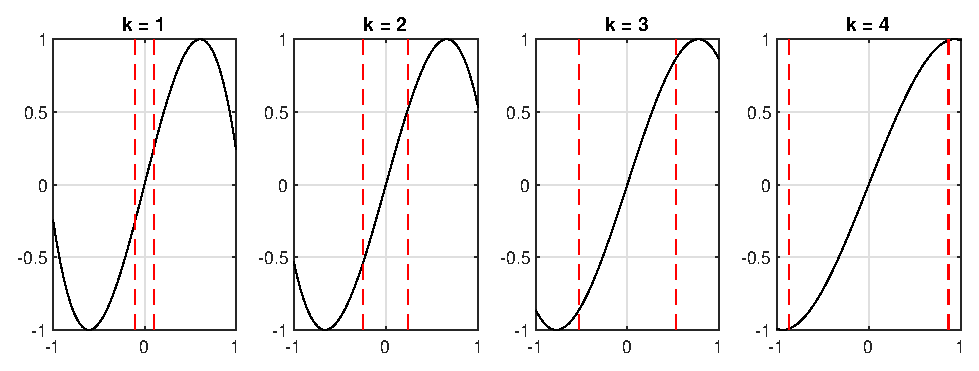
\includegraphics[width=\textwidth,height=\textheight,keepaspectratio]{figures/chapter_3/COMPSIGNiterationfunctions.eps}
   \caption{Iteration functions $g_k$ for the scaled Newton-Schulz iterates \eqref{deltak}. In each plot, the dotted red lines show the values of $\pm \delta_{k-1}$, starting with $\delta_0=\delta=0.1$.}
   \label{fig:compsigniterationfunctions}
\end{figure}

In particular, $\delta_k$ represents the value of $\delta$ used at the $(k+1)^{\text{st}}$ iteration to find the best cubic approximation to $C_{k+1} \sgn(x)$ on $X(\delta_k)$, as demonstrated in Figure \ref{fig:compsigniterationfunctions}. As a starting point, we have the formula
\[\ep_k:=\dfrac{E_k}{C_k}=\dfrac{1-\delta_k}{1+\delta_k},\]
which is the maximum uniform error $C_k^{-1}f_k-\sgn$. A comparison in the error of the scaled/unscaled Newton-Schulz iterates and the minimax approximation with respect to the degrees of freedom yields a striking result. Recall that the $k^{\text{th}}$ Newton-Schulz iterate (scaled or unscaled) has degree $3^k$, yet only $2k$ degrees of freedom\footnote{Each iteration function $g_k$ is an odd cubic polynomial, needing only two coefficients in terms of $\xi_k$ to be defined.}. However, the best approximation of degree $3^k$ requires $(3^k+1)/2$ degrees of freedom---half of a plain polynomial of degree $3^k$, since the best approximation is also an odd function). Therefore, the $k^\text{th}$ scaled or unscaled Newton-Schulz iterate has the same number of degrees of freedom as the minimax approximation of degree $4k-1$. 

\bigskip{}

\begin{figure}[t!]
\centering
   \includegraphics[width=0.7\textwidth,height=0.7\textheight,keepaspectratio]{figures/chapter_3/COMPSIGNvsBEST_DOFpoint1.eps}
   \caption{Comparison in the error of the Newton-Schulz, scaled Newton-Schulz and best approximants to $\sgn(x)$ on $X(\delta)$, where $\delta=0.1$, with respect to the degrees of freedom. The minimax is approximated using \texttt{polyvalA} and \texttt{polyfitA\_Lawson}\protect\footnotemark.}
   \label{fig:compsignvsbestDOF}
\end{figure}

Figure \ref{fig:compsignvsbestDOF} shows that the composite polynomial approximations are superior to the minimax with respect to degrees of freedom. Compared to \cite[Theorem 1]{Erem}, which shows that the minimax $p^*_m \in \Pee_{2m+1}$ to $\sgn(x)$ on $X(\delta)$ satisfies
\begin{align}
    \norm{p^*_m - \sgn}_{\infty,X(\delta)} \sim \dfrac{1-\delta}{\sqrt{\pi\delta}} m^{-1/2} \left(\dfrac{1-\delta}{1+\delta}\right)^m \label{eremboi}
\end{align}
as $m\to\infty$, we gain insight into why convergence of the minimax is much slower: despite being exponentially convergent, the term $\frac{1-\delta}{1+\delta}$ is very close to 1 for small values of $\delta$. A further observation from Figure \ref{fig:compsignvsbestDOF} is that, whereas the standard Newton-Schulz iterates perform worse than the minimax in the initial convergence phase, the scaled Newton-Schulz iterates are quick to outperform the minimax.

\bigskip{}

\footnotetext{Introduced by Brubeck, Nakatsukasa and Trefethen, these functions are adaptations of the standard \texttt{polyval} and \texttt{polyfit} methods---which fit polynomials to data using Vandermonde matrices---made stable by means of Arnoldi orthogonalisation. For details, see \cite{vandermonde}.}

\begin{figure}[t!]
\centering
   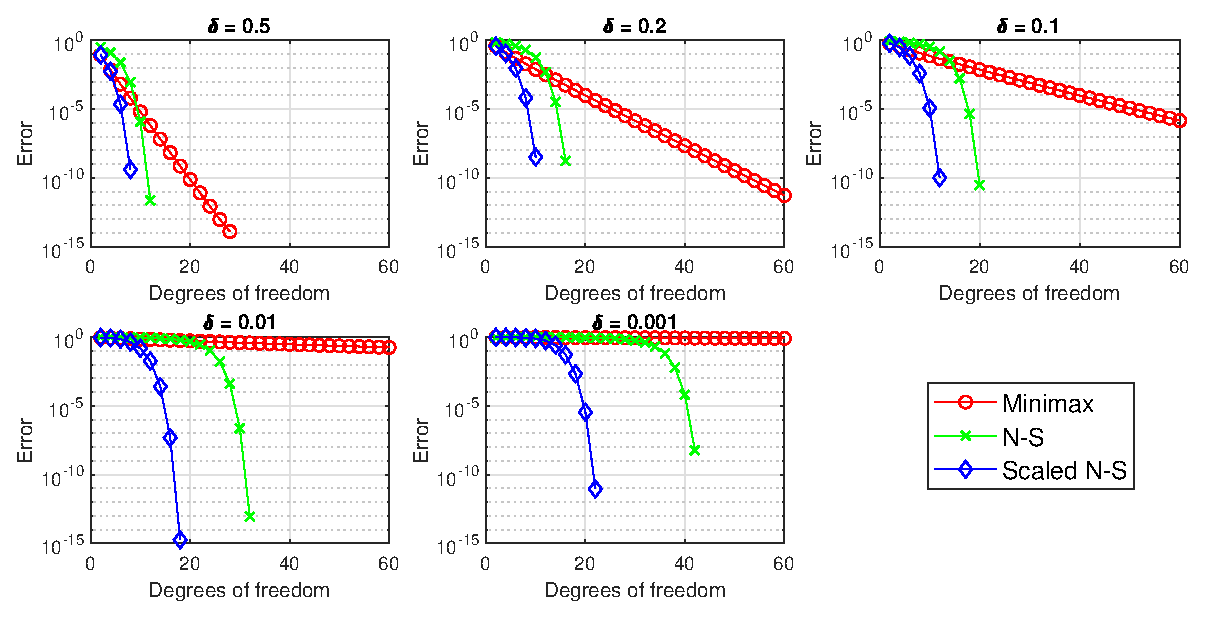
\includegraphics[width=\textwidth,height=\textheight,keepaspectratio]{figures/chapter_3/COMPSIGNvsBEST_DOF_MANY.eps}
   \caption{Error of the unscaled/scaled Newton-Schulz iterates and best approximants to $\sgn(x)$ on $X(\delta)$, with respect to the degrees of freedom, for different values of $\delta$.}
   \label{fig:compsignvsbestDOFmany}
\end{figure}

Comparisons in the error of all the approximations for different values of $\delta$ are shown in Figure \ref{fig:compsignvsbestDOFmany}. For increasingly small values of $\delta$, we observe that the number of iterations required by the unscaled Newton-Schulz iteration in the initial phase of convergence grows faster than that required by the scaled Newton-Schulz iteration. 

%\subsection{Approximating the number of iterations required in the initial convergence phase}

%In this subsection, we compute the approximate number of iterations required by both iterations to obtain an error of $\ep \approx 10^{-1}$, before embarking in some more rigourous analysis shortly. A simple Taylor expansion shows that 
%\[H(x) \sim \dfrac{3\sqrt{3}}{2}x + O(x^2)\] 
%as $x \to 0$, hence we have the approximate error
%\[\ep_k \sim \dfrac{1-C^k \delta}{1+C^k \delta}\]
%as $\delta \to 0$, where $C=3\sqrt3/2$. This is in contrast to the unscaled Newton-Schulz iterates $\tilde{f}_k(x)=g(\tilde{f}_{k-1}(x))$, where $g$ is as in \eqref{scalarNSsign}, which have error $\tilde{\ep}_k:=\tilde{f}_k(\delta)$. By the remark after \cite[Theorem 2.2]{chen}, $\tilde{\ep}_k$ is approximately
%\[\tilde{\ep}_k \sim 1-\left(\dfrac{3}{2}\right)^k \delta\]
%as $\delta \to 0$. Using these relations, we can confirm our first observation about Figure \ref{fig:compsignvsbestDOFmany}, namely that the number of extra iterations required by the unscaled Newton-Schulz approximation grows faster than that required by scaled Newton-Schulz approximation in the initial convergence phase, as $\delta \to 0$. Rearranging for the number of iterations $k$, we find for the scaled Newton-Schulz approximation that 
%\begin{align}
%    k \sim \dfrac{\log\frac{1-\ep}{1+\ep}+\log\frac{1}{\delta}}{\log \frac{3\sqrt{3}}{2}}\label{approx11}
%\end{align}
%iterates are needed for an error of $\ep$, and similarly for the unscaled Newton-Schulz approximation we require
%\begin{align}
%    k \sim \dfrac{\log(1-\ep)+\log\frac{1}{\delta}}{\log \frac{3}{2}}\label{approx22}
%\end{align}
%iterations for an error of $\ep$ in the initial convergence phase. We illustrate this remark in Figure \ref{fig:approxnumberofiterates}, which plots $\delta$ against the approximate number of iterations required by the scaled \eqref{approx11} and unscaled \eqref{approx22} Newton-Schulz iterates to obtain an error of $\ep=0.1$, which is roughly where the convergence seems to start becoming quadratic. Our figure is surprisingly accurate, after cross-checking the number of iterations for $\delta=10^{-p}$, where $p=1,2,3$, with Figure \ref{fig:compsignvsbestDOFmany} (note that DOFs = 2$*$iterations).

%\begin{figure}[t!]
%\centering
%   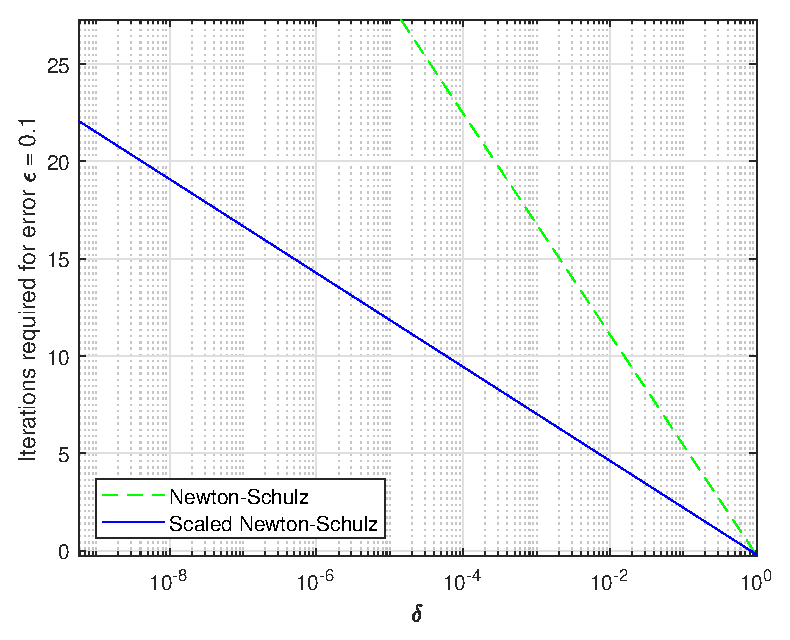
\includegraphics[width=0.7\textwidth,height=0.7\textheight,keepaspectratio]{asymptotic_iteratenumberDOF.eps}
%Newton-Schulz iterations to $\sgn(x)$ to obtain an accuracy of $\ep=0.1$.}
%   \label{fig:approxnumberofiterates}
%\end{figure}

\subsection{Deriving a lower bound for the number of iterations}

To obtain a lower bound for the number of iterations needed to obtain a given accuracy $\ep>0$ for arbitrary $\delta$, it thus seems reasonable to split the convergence analysis into the two phases mentioned in Section \ref{improvednewtonsection}: the initial convergence phase where we reduce the error to a suitably small value, and the asymptotic phase thereafter. We do this by taking inspiration from the analysis conducted by Gawlik and Nakatsukasa (see \cite{Yuji}, or Appendix \ref{compratappendix}).

\bigskip{}

Let $\ep>0$ be the required accuracy. In this subsection, we appropriately select a constant $\delta^* \in (1/e,1)$ and split the convergence into the the following three steps:
\begin{enumerate}
    \item[(1)] find $k_1$ such that $\delta_{k_1} \geq 1/e;$
    \item[(2)] find $k_2$ such that $\delta_{k_1+k_2} \geq \delta^*$;
    \item[(3)] find $k_3$ such that $\ep_{k_1+k_2+k_3} \leq \ep$.
\end{enumerate}

\textbf{Step 1.} Let $k_1$ be the smallest $k$ such that $\delta_k \geq 1/e$. By substituting $x=\delta$ in \eqref{deltak}, we obtain the recursion $\delta_{k+1}=H(\delta_k)$, where
\begin{align}
H(x)=\dfrac{3\sqrt{3}}{2}x\left(\dfrac{1+x}{(1+x+x^2)^{3/2}}\right). \label{hfunction}
\end{align}
A lower bound on $k_1$ is then readily obtained using the following observation.

\begin{lemma}\label{bigdeltalemma}
Let $\delta=\delta_0\in(0,1)$, and define $\delta_{k+1}=H(\delta_k)$ using \eqref{hfunction}. Then
\[\delta_k > \Delta^k \delta\]
for all $k\leq k_1$, where
\[\Delta = \dfrac{H(1/e)}{1/e}\approx 1.928.\]
\end{lemma}

\begin{proof}
Since $H(x)/x$ is strictly decreasing for $x>0$, and $\{\delta_k\}_{k\geq 0}$ is an increasing sequence, it follows that the ratio $\delta_{k+1}/\delta_k$ is also strictly decreasing. In particular, for all $k < k_1$, we have
\begin{align*}
    \dfrac{\delta_{k+1}}{\delta_k}> \dfrac{H(1/e)}{1/e}=\Delta.
\end{align*}
Inductively, it follows that
\[\delta_{k}  >\Delta^{k}\delta_0 = \Delta^{k}\delta\]
for all $k \leq k_1$, as required.
\end{proof}
Choosing $k=k_1$ in Lemma \ref{bigdeltalemma}, we find that $\delta_{k_1}\geq 1/e$ whenever $\Delta^{k_1}\delta\geq 1/e$. As a result, we obtain the lower bound
\[k_1 \geq \dfrac{\log \frac{1}{\delta}-1}{\log\Delta}.\]

%\begin{lemma}\label{taylolemma}
%Given $\delta\in (0,1)$ and $p \in \Pee_3$ defined by \eqref{xis}, we have
%\begin{align}
%    p(x) > \dfrac{3-\delta^2/\xi^2}{2\xi}x,\label{geom}
%\end{align}
%for all $x \in (0,\delta)$.
%\end{lemma}

%\begin{proof}
%This follows trivially, since by definition
%\[p(x)-\dfrac{3-\delta^2/\xi^2}{2\xi}x  = \dfrac{x}{2\xi^3}(\delta^2-x^2) > 0\]
%for all $x \in(0,\delta)$. Geometrically, we interpret the right-hand side of \eqref{geom} as the line through the %origin and $(\delta,p(\delta))$, which lies strictly below $p$ on $(0,\delta)$.
%\end{proof}

%Choosing $\delta=\delta_{k_1}$ and $x=\delta_k$ in Lemma \ref{taylolemma}, where $k_1$ is such that %$\delta_{k_1}\geq 1/e$ and $k < k_1$, we see that
%\[\delta_{k+1} > \dfrac{3-\delta^2_k/\xi_k^2}{2\xi_k} \delta_k\]
%for all $k < k_1$. By definition, this is simply
%\[H(x) > \dfrac{3\sqrt{3}}{2}\left(\dfrac{1+\delta_k}{(1+\delta_k+\delta_k^2)^{3/2}}\right)x.\]
%We have $\delta_{k_1} \gtrsim 1/e$ when
%\[\left(\dfrac{3\sqrt{3}}{2}\right)^{k_1}\delta \gtrsim \dfrac{1}{e},\]
%or equivalently
%\[k_1 \gtrsim \dfrac{\log \frac{1}{\delta}-1}{\log \frac{3\sqrt{3}}{2}}.\]

\textbf{Step 2.} This step no longer depends on $\ep$ or $\delta$, so $k_2$ is a constant. We select $\delta^*$ such that the following lemma holds, as this will help us in step 3. Firstly, define 
\[G(x)=\frac{2\sqrt{x}}{1+x}.\] 

\begin{lemma}\label{hh}
There is $\delta^*\in(0,1)$ such that for every $\delta \in [\delta^*,1]$, there holds
\[\dfrac{1-G(\delta)}{1+G(\delta)}\leq \left(\dfrac{1-\delta}{1+\delta}\right)^2.\]
\end{lemma}

\begin{proof}
As in \cite[Lemma 4.1]{Yuji}. It is shown in \cite[Theorem 3.2]{Gawlik} that the sequence defined by $\alpha_{k+1}=G(\alpha_k)$, where $\alpha_0 \in (0,1)$, is increasing to 1 as $k\to\infty$, and
\[\dfrac{1-G(\alpha_k)}{1+G(\alpha_k)}=\dfrac{1-\alpha_{k+1}}{1+\alpha_{k+1}}=\dfrac{1}{4}\left(\dfrac{1-\alpha_k}{1+\alpha_k}\right)^2+o\left(\left(\dfrac{1-\alpha_k}{1+\alpha_k}\right)^2\right).\]
It follows that
\[\dfrac{1-G(\alpha)}{1+G(\alpha)}\bigg/ \left(\dfrac{1-\alpha}{1+\alpha}\right)^2 \to \dfrac{1}{4}\]
as $\alpha \to 1^-$. Hence $\frac{1-G(\alpha)}{1+G(\alpha)}\big/ \left(\frac{1-\alpha}{1+\alpha}\right)^2$ is bounded by 1 for $\alpha$ sufficiently close to 1.
\end{proof}

\textbf{Step 3.} Let $k_3$ be such that $\ep_{k_1+k_2+k_3} \leq \ep$. To find a lower bound on $k_3$, we will use one final technical lemma.

\begin{lemma}\label{finallemma}
For every $x\in[0,1]$, we have
\[H(x)\leq G(x).\]
\end{lemma}

\begin{proof}
Re-arranging the desired inequality, it suffices to show that
\[J(x):=\dfrac{x(1+x)^4}{(1+x+x^2)^3} \leq \dfrac{16}{27}\]
for all $x \in [0,1]$. Differentiating $J$, we find that
\[J'(x) = \dfrac{(1-x)(x^2+4x+1)(1+x)^3}{(1+x+x^2)^4}\geq 0\]
on $[0,1]$, with equality only when $x=1$. Hence $J$ is bounded by $J(1)=16/27$.
\end{proof}

It follows by Lemma \ref{finallemma} that
\[\dfrac{1-H(\delta_{k})}{1+H(\delta_{k})} \leq \dfrac{1-G(\delta_{k})}{1+G(\delta_{k})},\]
since $x\mapsto \frac{1-x}{1+x}$ is decreasing. By our choice of $\delta^*$, we apply Lemma \ref{hh} to obtain
\[\dfrac{1-\delta_{k+1}}{1+\delta_{k+1}}=\dfrac{1-H(\delta_{k})}{1+H(\delta_{k})} \leq \dfrac{1-G(\delta_{k})}{1+G(\delta_{k})}\leq \left(\dfrac{1-\delta_{k}}{1+\delta_{k}}\right)^2,\]
for $k\geq k_1+k_2$. Inductively, we obtain
\[\dfrac{1-\delta_{k_1+k_2+k}}{1+\delta_{k_1+k_2+k}} \leq \left(\dfrac{1-\delta^*}{1+\delta^*}\right)^{2^k},\]
so we have $\ep_{k_1+k_2+k_3} \leq \ep$ if
\[\left(\dfrac{1-\delta^*}{1+\delta^*}\right)^{2^{k_3}} \leq \ep.\]
Taking logarithms twice, we find
\[k_3 \geq \dfrac{\log\log\frac{1}{\ep}-\log\log\frac{1+\delta^*}{1-\delta^*}}{\log 2}.\]
Combining the all steps, we have that $\ep_k \leq \ep$ when 
\begin{align}
    k \geq  \dfrac{\log \frac{1}{\delta}}{\log \Delta} + \tilde{k}_2 +\dfrac{\log\log\frac{1}{\ep}}{\log 2}, \label{NUMBERITERS}
\end{align}
where $\tilde{k}_2$ is a constant such that
\[\tilde{k}_2 = k_2 - \dfrac{1}{\log \Delta}-\dfrac{\log\log\frac{1+\delta^*}{1-\delta^*}}{\log 2}.\]

%To illustrate the analysis above, we pick a value of $k$ and compute the value of $\delta \in (0,1)$, and thus $\ep_k=\frac{1-\delta_k}{1+\delta_k}$ also, such that the scaled Newton-Schulz iteration $C_k^{-1}f_k$ has approximate error
%\[\norm{C_k^{-1}f_k -\sgn}_{\infty, X(\delta)} \lesssim \ep_k.\]
%Figure \ref{?} demonstrates this for different values of $k$.

%\subsection{Asymptotic behaviour}

%The simplest observation we can make about the scaled Newton-Schulz iterates is what happens as $k \to \infty$. Since $\{\delta_k\}_{k\geq 1}$ is bounded above by $1$, and strictly increasing by Lemma \ref{tekky}, we have $\delta_k \to 1$ as $k\to\infty$. Hence $g_k \to g_$, where
%\[g(x) = \dfrac{x}{2}\left(3-x^2\right),\]
%since $\xi_k \to 1$ also; note that $g$ is precisely the Newton-Schulz iteration function for approximating $\sgn(x)$. Indeed, this shows that convergence is quadratic because $\ep_k \to 0$ quadratically if $\delta_k \to 1$ quadratically, and it follows by similar reasoning to \cite[Theorem 4.2]{chen} we can show that
%\[\lim_{x\to 1}\dfrac{|H(x)-1|}{|x-1|^2} = \lim_{x\to 1} \frac{\left|\frac{3\sqrt{3}}{2}x\left(\frac{1+x}{(1+x+x^{2})^{3/2}}\right)-1\right|}{\left|x-1\right|^{2}}= \dfrac{3}{8}.\]

\subsection{Convergence with respect to degrees of freedom}

In Figure \ref{fig:compsignvsbestDOFmany}, we saw how the scaled Newton-Schulz approximation outperformed the minimax with respect to degrees of freedom. While \eqref{eremboi} shows that the minimax converges exponentially with respect to degrees of freedom, we can use \eqref{NUMBERITERS} to prove that, for any fixed value of $\delta$, the convergence of the scaled Newton-Schulz approximation is \textit{doubly exponential} with respect to degrees of freedom. 

\begin{thm}
Let $\delta \in (0,1)$, and $f_k \in \Pee_{(k,3)}^{\text{comp}}$ be the scaled Newton-Schulz iteration defined by \eqref{deltak}. Then there exist $C_1,C_2>0$ such that
\[\norm{f_k-C_k\emph{\sgn}}_{\infty,X(\delta)} = O(\exp(-C_1 \exp(C_2 d))),\]
where $d=2k$ denotes the number of degrees of freedom of $f_k$.
\end{thm}

\begin{proof}
Equivalently we can show that $\ep_k$, the maximum uniform error of $C_k^{-1}f_k$ to $\sgn$ on $X(\delta)$, is $O(\exp(-C_1 \exp(C_2 d)))$. Increasing $\tilde{k}_2$ until the right-hand side of \eqref{NUMBERITERS} is an integer, and recalling that $f_k$ has degree $3^k$, we find that the degree $n$ of $f_k$ achieving accuracy $\ep_k \leq \ep$, where $\ep >0$, satisfies
\[\dfrac{\log n}{\log 3}=\dfrac{\log \frac{1}{\delta}}{\log \Delta} + \tilde{k}_2 +\dfrac{\log\log \frac{1}{\ep}}{\log 2}.\]
We rearrange this to obtain a bound on $\ep$ as follows:
\begin{align*}
    \log\log\frac{1}{\ep} &= \log 2 \left(\dfrac{\log n}{\log 3}-\dfrac{\log\frac{1}{\delta}}{\log \Delta}-\tilde{k}_2\right)\\
    &=C\log n + D,
\end{align*}
where $C=\log_3 2$ and $D=\log 2\left(\frac{\log\delta}{\log\Delta} - \tilde{k}_2\right)$. Then
\[\log \dfrac{1}{\ep}=\exp(C\log n+D) = \tilde{D} n^C,\]
where $\tilde{D}=e^D$. Finally, we obtain
\begin{align*}
    \ep &= \exp(-\tilde{D}n^C)\\
    &=\exp(-\tilde{D}\exp(C\log n)) \\
    &= \exp(-\tilde{D}\exp(\tilde{C}d)),
\end{align*}
where $\tilde{C}=\frac{1}{2}C\log 3$, since $d=2k=2\log n /\log 3$. Hence the convergence of the scaled Newton-Schulz iteration is doubly exponential with respect to $d$.
\end{proof}

% CHAPTER
\chapter{Composite polynomial approximation to \texorpdfstring{$\sqrt{x}$}{sqrt(x)}} \label{sqrtchapter}

\section{Zolotarev functions and matrix roots revisited}

The Zolotarev functions \eqref{zolotarevfn} have a diverse range of applications beyond the sign function, as seen in \cite[Section 3.7]{YujiZolotFreund} and \cite[Chapter 9]{akhiezer}. One particularly interesting feature is that best rational approximations to the square root on $[\delta^2,1]$, in the relative sense, are closely related to the Zolotarev functions: if
\[Z_{2r+1}(x;\delta) = x\dfrac{P_r(x^2)}{Q_r(x^2)}, \qquad P_r, Q_r \in \Pee_r,\]
then $Q_r(x)/P_r(x)$ is a rational best approximation to $\sqrt{x}$. Figure \ref{fig:ZOLOT_SQRT} illustrates the first few iterates for $\delta=0.1$. 

\bigskip{}

In recent literature, the Zolotarev functions have been used to construct iterations for computing the principal square root of a matrix \cite{Gawlik,ZolotGawlik}. The matrix square root is perhaps the most widely studied matrix function---a range of iterative procedures exist for the approximation of the matrix square root, and they are well-documented in \cite[Section 6.3]{Higham}. Beyond Newton's Method, we can also obtain a large class of iterations\footnote{Details can be found in the paper of Higham, Mackey, Mackey \& Tisseur \cite[Theorem 4.5]{highamgroups}.} for the principal square root from the matrix sign function, by means of the identity
\[\sgn\left(\begin{bmatrix} 0 & A \\ I & 0 \end{bmatrix}\right)=\begin{bmatrix} 0 & A^{1/2} \\ A^{-1/2} & 0 \end{bmatrix},\]
first noted by Higham in \cite{HighamStable}. Clearly there are deep connections between the sign and square root functions, and we use the above observations as motivation for assesses the connection between $\sgn(x)$ and $\sqrt{x}$ in the setting of polynomial approximations. The following example relates their best approximations over previously considered intervals.

\begin{figure}[t!]
\centering
   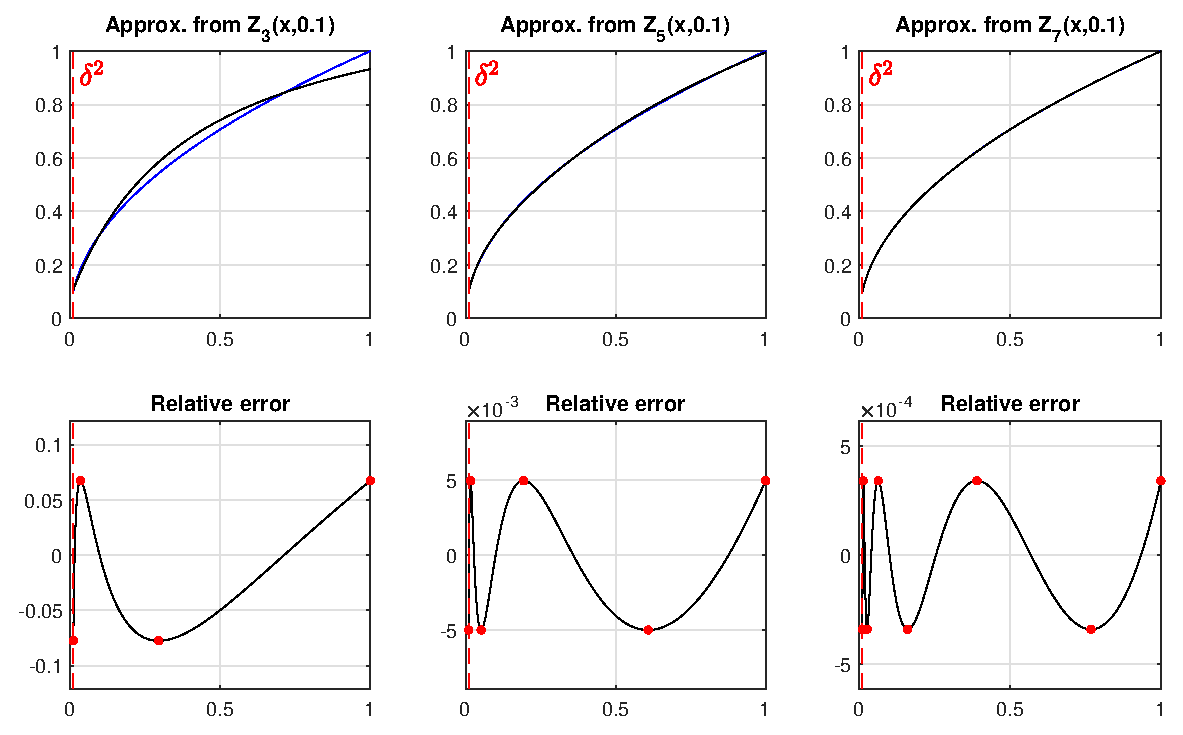
\includegraphics[width=\textwidth,height=\textheight,keepaspectratio]{figures/chapter_4/ZOLOTAREV_SQRT.eps}
   \caption{Approximations to $\sqrt{x}$ on $[\delta^2,1]$  for $\delta=0.03$, derived from the Zolotarev functions $Z_{2r+1}(x;\delta)$. The corresponding relative error is sketched below each plot, which equioscillates between $2r+2$ extrema in each case.}
   \label{fig:ZOLOT_SQRT}
\end{figure}

\begin{ex}\label{besties}
Consider the function $\sgn(x)$ on $X(\delta)$. Since $\sgn$ is odd, and $X(\delta)$ is symmetric about the origin, it follows by the remark after Lemma \ref{symm} that the best uniform polynomial approximation to $\sgn(x)$ on $X(\delta)$ is the best odd approximation $p^*(x)=xp(x^2)$ on $[\delta,1]$. Moreover, since $\sgn(x)=x/\sqrt{x^2}$ we can write the uniform error $\norm{\sgn-p^*}_{\infty,X(\delta)}$ as
\[\sup_{x\in [\delta,1]}|1 - xp(x^2)| = \sup_{x\in[\delta^2,1]}\left|\dfrac{xp(x)-\sqrt x}{\sqrt x}\right|.\]
That is, if the best uniform approximation to $\sgn(x)$ on $X(\delta)$ is $xp(x^2)$, then the best relative approximation to $\sqrt{x}$ on $[\delta^2,1]$ is $xp(x)$.
\end{ex}

Motivated by the connections between best approximations to $\sgn(x)$ and $\sqrt{x}$, this chapter attempts to use our scaled Newton-Schulz approximation to $\sgn(x)$ to generate a composite approximation to $\sqrt{x}$.

\section{Deriving an approximation from scaled Newton-Schulz iterates}

Recall the scaled Newton-Schulz approximation to $\sgn(x)$ on $X(\delta)$, given by
\begin{align}
    f_{k+1}(x)=\dfrac{f_k(x)}{2\xi_{k+1}}\left(3-\dfrac{f_k(x)^2}{\xi_{k+1}^2}\right), \qquad \xi_{k+1} = \sqrt{\dfrac{1+f_{k}(\delta)+f_{k}(\delta)^2}{3}}\label{forsqrt}
\end{align}
for $k\geq 0$, with initial guess $f_0(x)=x$. Here the $f_k$ approximate $C_k \sgn(x)$, where $C_k=(1+f_k(\delta))/2$. Each $f_k$ is an odd function, hence by Lemma \ref{symm} we can write $f_k(x)=xh_k(x^2)$ for some polynomial $h_k$. This observation allows us to derive a square root approximation, which we illustrate in Figure \ref{fig:compsqrt3}.

\begin{thm}
Let $\delta \in (0,1)$, $f_k \in \Pee_{(k,3)}^{\text{comp}}$ be the scaled Newton-Schulz iteration to $C_k \sgn (x)$ defined by \eqref{forsqrt}, and $E_k$ be the maximum uniform error. Writing $f_k(x)=xh_k(x^2)$, the iterates $F_k(x)=xh_k(x)$ provide a composite approximation 
\[F_{k+1}(x) = \dfrac{F_k(x)}{2\xi_{k+1}}\left(3-\dfrac{F_k(x)^2}{x\xi_{k+1}^2}\right), \qquad \xi_k = \sqrt{\dfrac{\delta^2+\delta F_{k-1}(\delta^2) + F_{k-1}(\delta^2)^2}{3\delta^2}} \]
to $\sqrt{x}$, for which
\[\norm{F_k - C_k\sqrt{x}}_{\infty,[\delta^2,1]} \leq E_k.\]
\end{thm}

\begin{proof}
The error bound follows from the fact that
\begin{align*}
    \norm{\sgn-C_k^{-1}f_k}_{\infty,X(\delta)}&= \norm{\dfrac{C_k x\sgn-xf_k}{C_k x}}_{\infty,X(\delta)}\\
    &=\norm{\dfrac{C_k\sqrt{x}-F_k}{C_k\sqrt{x}}}_{\infty,[\delta^2,1]}\\
    & \geq C_k^{-1} \norm{C_k\sqrt{x}-F_k}_{\infty,[\delta^2,1]},
\end{align*}
similar to Example \ref{besties}. To obtain a recursion for the $F_k$, we first note that
\[F_k(\delta^2)=\delta^2 h_k(\delta^2) = \delta f_k(\delta),\]
so we can rewrite $\xi_k$ in terms of the $F_{k-1}$, namely
\[\xi_k = \sqrt{\dfrac{\delta^2+\delta F_{k-1}(\delta^2) + F_{k-1}(\delta^2)^2}{3\delta^2}}.\]
We can derive a sequence for the $F_k$, since by \eqref{forsqrt} we have
\[xh_{k+1}(x^2)=\dfrac{xh_k(x^2)}{2\xi_{k+1}}\left(3-\dfrac{x^2h_k(x^2)^2}{\xi_{k+1}^2}\right),\]
hence a recursion for the $h_k$ is given by
\[h_{k+1}(x) = \dfrac{h_k(x)}{2\xi_{k+1}}\left(3-\dfrac{xh_k(x)^2}{\xi_{k+1}^2}\right).\]
Multiplying by $x$ gives
\begin{align}
    F_{k+1}(x) = \dfrac{F_k(x)}{2\xi_{k+1}}\left(3-\dfrac{F_k(x)^2}{x\xi_{k+1}^2}\right), \label{comprelsqrt}
\end{align}
as required.
\end{proof}

\begin{figure}[t!]
\centering
   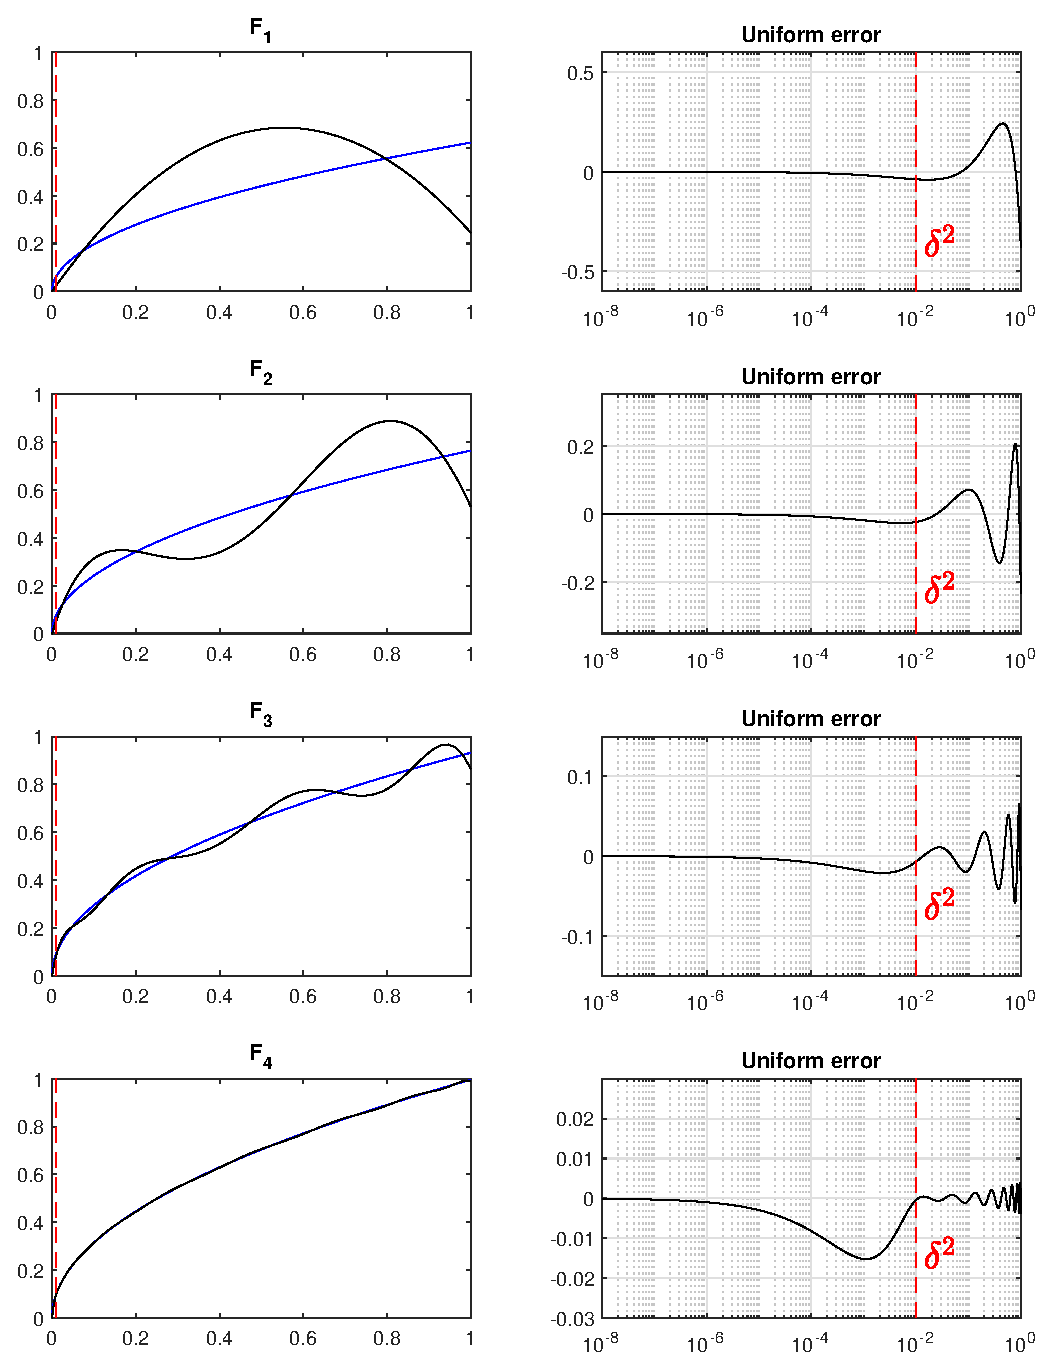
\includegraphics[width=\textwidth,height=\textheight,keepaspectratio]{figures/chapter_4/COMPSQRT_4ITERS_UNIF.eps}
   \caption{Composite polynomial approximations $F_k$ (black) to $C_k\sqrt{x}$ (blue) on $[0,1]$, choosing $\delta=0.1$ (red dashed line). The uniform errors are plotted beside each iteration. On $[\delta^2,1]$, the relative error will be identical to the uniform error the scaled Newton-Schulz iterates to the sign function on $X(\delta)$.}
   \label{fig:compsqrt3}
\end{figure}

\begin{rmk}
For any initial guess $F_0$ divisible by $x$, it follows inductively that $F_k$ is a polynomial for all $k$. This is a non-pure composite approximation to $C_k\sqrt{x}$ on $[\delta^2,1]$ in the relative sense, and the error analysis will thus fall largely in line with that of the previous chapter. Furthermore, the iteration \eqref{comprelsqrt} can be seen as a scaled version of the Alternative Newton iterates \eqref{altnewt} considered in the preliminary discussion, where once again the iteration function $G_k$ is such that $x$ is replaced by $x\xi_k^{-1}$. As such, we will refer to these as \textit{scaled Alternative Newton} iterates to $\sqrt{x}$.
\end{rmk}

\section{Observations of the scaled Alternative Newton iterates}

On the interval $[\delta^2,1]$, our convergence analysis follows largely as in the previous chapter due to Theorem 4.2. A natural question to ask is how convergence differs when considering the $F_k$ on the whole interval $[0,1]$. In particular, if we are allowed at most $k$ iterations, what is the value of $\delta$ that we should choose to minimise the error? The answer to this question is far from obvious, as Figures \ref{fig:scaled_alt1}-\ref{fig:scaled_alt4} illustrate. These figures compare the maximum error in the unscaled and scaled Alternative Newton iterates, alongside the standard Newton iteration. As we might have expected, the Newton iteration eventually outperforms the alternative iterations for all choices of $\delta$. What is unexpected is that for sufficiently small values of $\delta$, the scaled Alternative Newton approximation can even perform better than Newton's method. For instance, if we allow ourselves 10 iterations, it is more efficient to use our approximation with $\delta=0.001$ with the standard Newton iterates.

\begin{figure}[t!]
\centering
   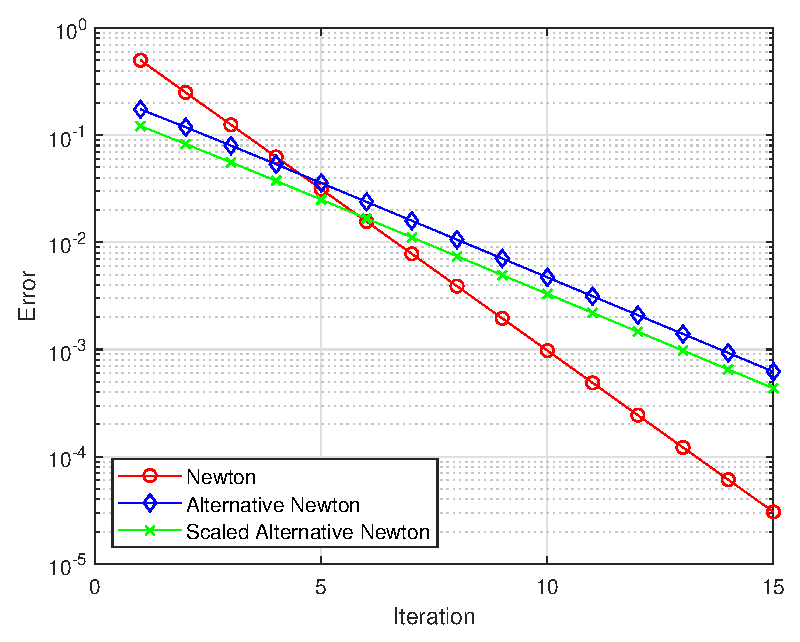
\includegraphics[width=0.7\textwidth,height=0.7\textheight,keepaspectratio]{figures/chapter_4/AN_vs_SAN_0p5.eps}
   \caption{Comparison of the error in Newton, Alternative Newton and scaled Alternative Newton iterates to $\sqrt{x}$ on $[0,1]$, with a choice of $\delta=0.5$.}
   \label{fig:scaled_alt1}
\end{figure}

\begin{figure}[t!]
\centering
   \includegraphics[width=0.7\textwidth,height=0.7\textheight,keepaspectratio]{figures/chapter_4/AN_vs_SAN_0p1.eps}
   \caption{Comparison of the error in Newton, Alternative Newton and scaled Alternative Newton iterates to $\sqrt{x}$ on $[0,1]$, with a choice of $\delta=0.1$.}
   \label{fig:scaled_alt2}
\end{figure}

\begin{figure}[t!]
\centering
   \includegraphics[width=0.7\textwidth,height=0.7\textheight,keepaspectratio]{figures/chapter_4/AN_vs_SAN_0p01.eps}
   \caption{Comparison of the error in Newton, Alternative Newton and scaled Alternative Newton iterates to $\sqrt{x}$ on $[0,1]$, with a choice of $\delta=0.01$.}
   \label{fig:scaled_alt3}
\end{figure}

\begin{figure}[t!]
\centering
   \includegraphics[width=0.7\textwidth,height=0.7\textheight,keepaspectratio]{figures/chapter_4/AN_vs_SAN_0p001.eps}
   \caption{Comparison of the error in Newton, Alternative Newton and scaled Alternative Newton iterates to $\sqrt{x}$ on $[0,1]$, with a choice of $\delta=0.001$.}
   \label{fig:scaled_alt4}
\end{figure}
% CHAPTER
\chapter{Conclusion}

Motivated by the recursive optimality property of the Zolotarev functions, we constructed a composite polynomial approximation to the scalar sign function on $[-1,-\delta]\cup[\delta,1]$ using a greedy iterative process. Although our construction was not optimal, we showed that it was equivalent to a scaled variant of the Newton-Schulz method for approximating the sign function, where the scaling at each iteration depended on the value of the extremal point of the iteration function. We noted that, when compared to the minimax approximation with respect to degrees of freedom, the scaled Newton-Schulz iteration was far superior. For a given $\delta$, a lower bound number of iterations needed to obtain a given accuracy $\ep>0$ was derived, in a similar manner to the work of Nakatsukasa and Gawlik \cite{Yuji}, and this bound was used to show that the converge of the scaled-Newton Schulz iteration is doubly exponential with respect to the degrees of freedom.

\bigskip{}

We also proved that the scaled Newton-Schulz iteration can be transformed into a composite approximation for the square root function whose error on $[\delta^2,1]$ is bounded by the error in the sign functino approximation; the iteration we derived produces polynomial iterates for any initial guess divisible by $x$. This approximation was shown to be equivalent and superior to a scaled variant of Newton's Method---one in which a different algebraic equation was initially considered, in order to avoid iterates dividing by their predecessor and hence generating rational approximations. 

\bigskip{}



\section{Where does this project lead?}

Throughout this dissertation, many potential avenues were unlocked for further research. On multiple occasions, we drew attention to how composite polynomial and rational approximations are used to compute matrix functions, yet this is an area which we purposefully avoided to focus our work on gleaning results at a scalar level. The power and limitations of our constructed approximations when evaluated at a matrix argument are yet to be fully explored.

\bigskip{}

With regards to the scaled Newton-Schulz iteration, the following two questions were left unsolved. Firstly, while the iteration appears to perform well in the space of composite polynomials, it is unclear whether or not our construction is indeed the best approximation with respect to the space $\Pee_{(k,3)}^{\text{comp}}$. For example, can we find suboptimal iteration functions $\tilde{g}_i$ such that, when composed, $\tilde{g}_2(\tilde{g}_1(x))$ is a better approximation to the sign function than $g_2(g_1(x))$? Moreover, what if we considered greedy approximations comprising of higher-degree polynomials, such as $\Pee_{(k,5)}^{\text{comp}}$ or $\Pee_{(k,7)}^{\text{comp}}$? At what point does the computational cost arising from the degree of the composed polynomials cease to be optimal? 

\bigskip{}

Finally, and most importantly, we wish to continue the analysis of the scaled Alternative Newton iteration to $\sqrt{x}$ beyond the submission of this dissertation. From the perspective of rational functions, we know that there is a composite approximation whose convergence is \textit{doubly exponential} with respect to the degrees of freedom \cite{Yuji}, and Figures 4.3-4.6 seem to suggest that convergence will be at least exponential in the polynomial setting.
%APPENDIX
\begin{appendices}

\chapter{Results for composite rational functions}\label{compratappendix}

This appendix will contain results relating to composite rational functions. As such, we will briefly discuss some definitions and examples---similar to those seen in the preliminary discussion in a polynomial setting---involving rational functions.

\section{Composite rational functions and degrees of freedom} 

\begin{defn}
The \textit{degrees of freedom} of a rational function $r_{m,n} \in \Arr_{m,n}$ is the number of parameters required to completely determine $r_{m,n}$. We say that $r_{m,n}$ is a \textit{plain rational function} if $r_{m,n}$ has $m+n+1$ degrees of freedom, i.e.
\[r_{m,n}(x) = \dfrac{\sum_{k=0}^m \alpha_k x^k}{1+\sum_{k=1}^n \beta_k x^k},\]
for some independent scalars $\alpha_k, \beta_k \in \R$.
\end{defn}

\begin{defn}\label{compratdef}
A bivariate rational function $r(x,y)$ is said to be of type $(m,n)$ if $r(x,x) \in \Arr_{m,n}$. A rational function $r(x)$ is said to be \textit{$(k,m,n)$-composite} if
\begin{align}
    r(x) = r_k(x,r_{k-1}(x,r_{k-2}(\cdots(x,r_1(x,1))))) \label{rat}
\end{align}
for bivariate rational functions $r_i(x,y)$, $i=1,\dots,k$, each of type $(m,n)$. We say that a $(k,m,n)$-composite rational function is $pure$ if the $r_i(x,y)$ in \eqref{rat} are univariate, i.e. $r(x) = r_k(r_{k-1}(\cdots(r_1(x))))$.
\end{defn}

\begin{ex}
A rational function of the form \eqref{rat} has at most $k(m+n+1)$ degrees of freedom. In particular, a pure composite rational function of the form $r(x)=r_k(\cdots r_2(r_1(x)))$ with each $r_i$ of type $(n,n)$ is of type $(n^k,n^k)$, but has $d\approx 2kn$ degrees of freedom.
\end{ex}

Examples of composite rational functions we have encountered throughout this dissertation include the Newton iterates for the sign and square root functions, and more subtly the Zolotarev functions.

\section{Composite rational approximation to \texorpdfstring{$\sqrt{x}$}{sqrt(x)}}

The motivation for the novel part of this dissertation, namely the construction of a composite polynomial approximation to $\sqrt{x}$, stemmed from the work of Gawlik and Nakatsukasa \cite{Yuji} concerning the composite rational approximation of $x^{1/p}$ on $[\alpha^p,1]$ for some $\alpha \in (0,1)$. In this appendix, we present their results for $p=2$, and simplify proofs where possible. 

\begin{thm}\label{squareroot}
There exists $N \in \N$ such that for every integer $n \geq N$, there is a rational function $r \in \Arr_{n,n-1}([0,1])$, which is a composition of $\lfloor\log_2 n\rfloor+1$ type-$(2,1)$ rational functions, and a constant $C>0$ such that
\[\max_{x\in[0,1]}|r(x)-\sqrt{x}| \leq \exp(-C\sqrt{n}).\]
\end{thm}

Theorem \ref{squareroot} implies that the convergence of $r$ to $\sqrt{x}$ is \textit{doubly exponential} with respect to $d$, the number of degrees of freedom, as $n\to\infty$. That is, for constants $C_1,C_2>0$, the error is $O(\exp(-C_1\exp(C_2 d)))$, where $d\approx 4\log_2 n$. To prove Theorem \ref{squareroot}, we consider
\begin{align}
    f_{k+1}(x)=\dfrac{1}{2}\left(\sqrt{\alpha_k}f_k(x)+\dfrac{x}{\sqrt{\alpha_k} f_k(x)}\right), \qquad f_0(x)=1, \label{theiter}
\end{align}
where throughout this appendix we define the sequence $(\alpha_k)$ by 
\[\alpha_{k+1}=\dfrac{2\sqrt{\alpha_k}}{1+\alpha_k},\qquad \alpha_0=\alpha.\]
Note that $f_k$ is $(k,2,1)$-composite with 
\[r_j(x,y)=\dfrac{1}{2}\left(\dfrac{\alpha_{j-1}y^2+x}{\sqrt{\alpha_{j-1}}y}\right), \qquad j=1,\dots,k.\]
A simple induction shows that $f_k \in \Arr_{2^{k-1},2^{k-1}-1}$ for each $k\geq 1$. In what follows, we will approximate the square root function with the scaled functions
\[\tilde{f}_k(x)=\dfrac{2\alpha_k}{1+\alpha_k}f_k(x),\]
which in particular have the same number of degrees of freedom of the $f_k$. We will prove the following result, which will enable us to show that the $\tilde{f}_k$ converge to $\sqrt{x}$ at a doubly exponential rate with respect to the degrees of freedom.

\begin{thm}\label{fsquig}
For any $k \in \N$, $\alpha \in (0,1)$, there holds
\[\max_{x\in[0,1]}|\tilde{f}_k(x)-\sqrt{x}| \leq \max\left\{2\alpha,\dfrac{1-\alpha_k}{1+\alpha_k}\right\}.\]
\end{thm}

\subsection{Bounding the error on \texorpdfstring{$[0,\alpha^2]$}{[0,a2]}}

To prove Theorem \ref{fsquig}, we consider the error over $[0,\alpha^2]$ and $[\alpha^2,1]$ separately. In this section, we consider the first interval and prove the following error bound.

\begin{thm}\label{0bound}
For any $k \in \N$, $\alpha \in (0,1)$, there holds
\[\max_{x\in [0,\alpha^2]}|\tilde{f}_k(x)-\sqrt{x}|\leq 2\alpha.\]
\end{thm}

To prove this, we need a few lemmas. We first define the functions
\[s_\alpha(x):= \dfrac{2x\sqrt{\alpha}}{\alpha+x^2}, \qquad H(\alpha):= s_\alpha(\alpha) = \dfrac{2\sqrt{\alpha}}{1+\alpha}, \qquad g_k(x):= \dfrac{x}{f_k(x^2)},\]
and note that
\begin{align}
    H(\alpha_k)=\alpha_{k+1}, \qquad g_{k+1}(x) = s_{\alpha_k}(g_k(x)). \label{geekay}
\end{align}

\begin{lemma}\label{A3}
For any $\alpha \in (0,1)$, $x \in [0,\alpha]$, we have
\[0 \leq x s'_\alpha(x) \leq s_\alpha(x) \leq H(\alpha).\]
\end{lemma}

\begin{proof}
Since $s_\alpha$ is nondecreasing on $[0,\alpha]$, we have 
\[0\leq xs'_\alpha(x), \qquad s_\alpha(x) \leq H(\alpha).\]
Furthermore, we can compute
\[xs'_\alpha(x) = \left(\dfrac{\alpha-x^2}{\alpha+x^2}\right)\left(\dfrac{2x\sqrt{\alpha}}{\alpha+x^2}\right)\leq s_\alpha(x)\]
since $0\leq \frac{\alpha-x^2}{\alpha+x^2}\leq 1$ for all $x \in [0,\alpha] \subset [0,\sqrt{\alpha}]$. 
\end{proof}

\begin{lemma} \label{ggkk}
For any $k \in \N$, $\alpha \in (0,1)$, $x \in [0,\alpha]$, we have
\begin{align}
    0 \leq x g'_k(x) \leq g_k(x) \leq \alpha_k.\label{lem2}
\end{align}
\end{lemma}

\begin{proof}
By induction. The case $k=0$ is clear since $g_0(x)=x$ and $\alpha_0=\alpha$. Now assume that \eqref{lem2} holds for $k=n$. By \eqref{geekay}, we have
\[xg'_{n+1}(x)=xs'_{\alpha_n}(g_n(x))g'_n(x).\]
As $0\leq g_n(x)\leq \alpha_n$ by the induction hypothesis, Lemma \ref{A3} with $\alpha=\alpha_n$ implies that $xg'_{n+1}(x)\geq 0$ for $x \in [0,\alpha]$. The lemma further shows that
\[xg'_{n+1}(x) \leq s'_{\alpha_n}(g_n(x))g_n(x) \leq s_{\alpha_n}(g_n(x)) = g_{n+1}(x).\]
Finally, as noted in Lemma \ref{A3},
\[g_{n+1}(x) = s_{\alpha_n}(g_n(x)) \leq H(\alpha_n) = \alpha_{n+1},\]
which completes the inductive step.
\end{proof}

\begin{lemma}\label{finallem}
For any $k \in \N$, $\alpha \in (0,1)$, $x \in [0,\alpha^2]$, we have
\[0 < \tilde{f}_k(x) \leq \alpha(1+\ep_k), \qquad \text{where}\qquad  \ep_k=\dfrac{1-\alpha_k}{1+\alpha_k}.\]
\end{lemma}

%Induction: f_k > 0 easy, f_k non-decreasing ok: clear for k=0, assume y>x and show f_k+1(y) >= f_k+1(x) 

\begin{proof}
A simple induction shows that $f_k(x)>0$ is non-decreasing on $[0,\alpha^2]$ for every $k$. Writing $f_k(x^2)=x/g_k(x)$, we differentiate to obtain
\[2xf'_k(x^2) = \dfrac{g_k(x)-xg'_k(x)}{g_k(x)^2} \geq 0\]
by Lemma \ref{ggkk}. Hence $f'_k(x^2)\geq 0$ for $x \in [0,\alpha^2]$. Setting \eqref{theiter} at $x=0$ gives
\[f_{k+1}(0)=\dfrac{\sqrt{\alpha_k}}{2}f_k(0), \qquad f_0(0)=1,\]
so $0<f_k(0)\leq f_k(x)$ on $[0,\alpha^2]$ for every $k$, and so $0<\tilde{f}_k(x)\leq \tilde{f}_k(\alpha^2)$ as $\tilde{f}_k$ is a positive multiple of $f_k$. The upper bound on $\tilde{f}_k$ is obtained by \cite[Theorem 3.1]{Gawlik}, which provides the relative error bound
\[\max_{x\in[\alpha^2,1]}\dfrac{\tilde{f}_k(x)-\sqrt{x}}{\sqrt{x}}=\dfrac{1-\alpha_k}{1+\alpha_k}=\ep_k.\]
Taking $x=\alpha^2$ gives $\tilde{f}_k(\alpha^2) \leq \alpha(1+\ep_k)$, as required.
\end{proof}

We are now in a position to prove Theorem \ref{0bound}, from which we can quickly deduce the result of Theorem \ref{fsquig}.

\begin{proof}[Proof of Theorem \ref{0bound}]
By Lemma \ref{finallem}, we have for $x\in [0,\alpha^2]$
\begin{align*}
    |\tilde{f}_k(x)-\sqrt{x}| &\leq \max\{|\tilde{f}_k(x)|,|\sqrt{x}|\}\\
    &\leq \max\{\alpha(1+\ep_k),\alpha\}\\
    &=\alpha(1+\ep_k)\\
    &\leq 2\alpha,
\end{align*}
since $\ep_k \in (0,1)$. Thus $\max_{x\in[0,\alpha^2]}|\tilde{f}_k(x)-\sqrt{x}|\leq 2\alpha$, as required.
\end{proof}

\begin{proof}[Proof of Theorem \ref{fsquig}]
If we combine the result of \cite[Theorem 3.1]{Gawlik} with Theorem \ref{0bound}, we obtain
\begin{align*}
    \max_{x\in[0,1]}|\tilde{f}_k(x)-\sqrt{x}| &=\max\left\{2\alpha,\max_{x\in[\alpha^2,1]}|\tilde{f}_k(x)-\sqrt{x}|\right\}\\
    & \leq \max \left\{2\alpha,\max_{x\in[\alpha^2,1]}\left|\dfrac{\tilde{f}_k(x)-\sqrt{x}}{\sqrt{x}}\right|\right\}\\
    & = \max\left\{2\alpha,\dfrac{1-\alpha_k}{1+\alpha_k}\right\},
\end{align*}
as required.
\end{proof}

\subsection{Proof of Theorem \texorpdfstring{\ref{squareroot}}{(4.1)}}

Theorem \ref{fsquig} is used in \cite{Yuji} as a basis for the analysis of the convergence of $\tilde{f}_k$ to $\sqrt{x}$ on $[0,1]$, and ultimately proving Theorem \ref{squareroot}. Nakatsukasa and Gawlik take a constructive approach to determining, for arbitrary $\ep>0$, values of $\alpha$, $k$ such that $\max_{x\in[0,1]}|\tilde{f}_k(x)-\sqrt{x}|< \ep$. By Theorem \ref{fsquig}, we must have $\alpha \leq \ep/2$ and $k$ large enough such that $\ep_k \leq \ep$. We determine $k$ in three steps:

\begin{enumerate}
    \item[(1)] Find $k_1$ such that $\alpha_{k_1} \geq 1/e$;
    \item[(2)] Select $\alpha^* \in (1/e,1)$ and find $k_2$ such that $\alpha_{k_1+k_2} \geq \alpha^*$;
    \item[(3)] Find $k_3$ such that $\ep_{k_1+k_2+k_3}\leq \ep$. 
\end{enumerate}

%\begin{figure}[t!]
%\centering
%   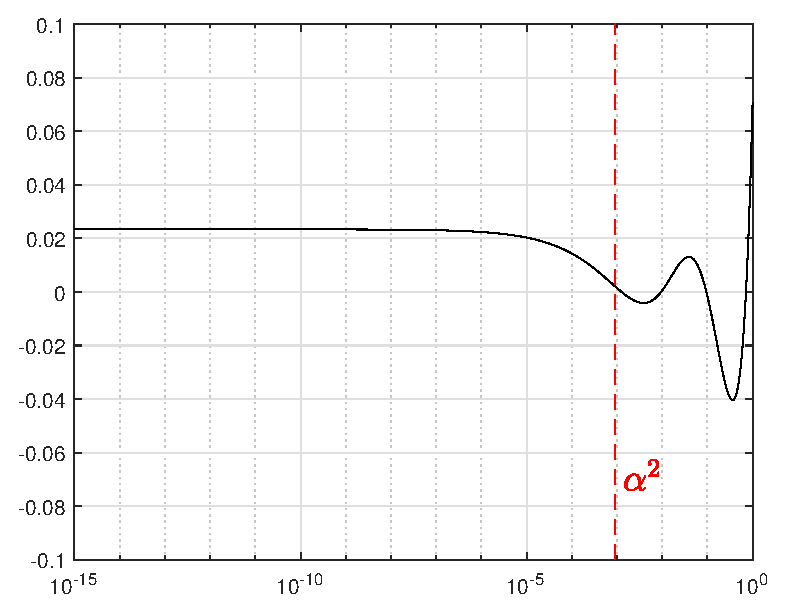
\includegraphics[scale=0.8]{Comp_sqrt_approx_withline.eps}
%   \caption{Error curve $E(x)=\tilde{f}_2(x)-\sqrt{x}$ for $\alpha=0.03$. Note that the error on $[0,\alpha^2]$ is bounded by that on $[\alpha^2,1]$, which is $\ep=2\alpha$.}
%   \label{fig:alpha}
%\end{figure}

Then $k\geq k_1+k_2+k_3$. The choice of $\alpha^*$ in step 2 is given by $\delta^*$ in Lemma \ref{hh}.

\bigskip{}

\textbf{Step 1.} To determine $k_1$ such that $\alpha_{k_1}\geq 1/e$, we first note that $\alpha_{k+1}> \sqrt{\alpha_k}$. To see this, we can argue by contradiction (a much simpler proof than that of Nakatsukasa and Gawlik). If $\alpha_{k+1} \leq \sqrt{\alpha_k}$, then
\begin{align*}
    \dfrac{2\sqrt{\alpha_k}}{1+\alpha_k}\leq \sqrt{\alpha_k} \qquad \Longrightarrow\qquad 2\sqrt{\alpha_k} &\leq \sqrt{\alpha_k} + \alpha_k\sqrt{\alpha_k} < 2\sqrt{\alpha_k},
\end{align*}
since $\alpha_k \in(0,1)$, a contradiction. Hence $\alpha_{k+1}>\sqrt{\alpha_k}$ for all $k$, so
\[\alpha_k \geq \alpha_0^{(1/2)^k}=\alpha^{(1/2)^k}.\]
Thus we will have $\alpha_{k_1}\geq 1/e$ if $\alpha^{(1/2)^{k_1}}\geq 1/e$, namely
\[k_1\geq \dfrac{\log\log \frac{1}{\alpha}}{\log 2}.\]
Since $\alpha\leq \ep/2$ is assumed, we can write a lower bound in terms of $\ep$, i.e.
\[k_1 \geq \dfrac{\log\log \frac{2}{\ep}}{\log 2}.\]

\textbf{Step 2.} We pick $\alpha^*$ such that the result of Lemma \ref{hh} holds. Note that $k_2$ is independent of $\ep$ and $\alpha$, hence constant.

\bigskip{}

\textbf{Step 3.} To determine $k_3$ such that $\ep_{k_1+k_2+k_3} \leq \ep$, we note that
\[\ep_{k+1}=\dfrac{1-H(\alpha_k)}{1+H(\alpha_k)}\leq \left(\dfrac{1-\alpha^*}{1+\alpha^*}\right)^2\]
for $k\geq k_1+k_2$ by Lemma \ref{hh}. In particular,
\[\ep_{k_1+k_2+k}\leq \ep_{k_1+k_2}^{2^k}\leq \left(\dfrac{1-\alpha^*}{1+\alpha^*}\right)^{2^k},\]
so $\ep_{k_1+k_2+k_3}\leq \ep$ if $k_3$ is chosen such that
\[k_3 \geq \dfrac{\log\log\frac{1}{\ep}-\log\log\frac{1+\alpha^*}{1-\alpha^*}}{\log 2}.\]

Combining the steps, we find that $\max_{x\in[0,1]}|\tilde{f}_k(x)-\sqrt{x}|< \ep$ when
\[k \geq \dfrac{\log\log\frac{2}{\ep}}{\log 2} + k_2 + \dfrac{\log\log\frac{1}{\ep}-\log\log\frac{1+\alpha^*}{1-\alpha^*}}{\log 2}.\]

We now prove Theorem \ref{squareroot}, simplifying the version provided in \cite{Yuji}.

\begin{proof}[Proof of Theorem \ref{squareroot}]
As previously mentioned, $\tilde{f}_k$ will be a type $(2^{k-1},2^{k-1}-1)$ rational function. Define 
\[\tilde{k}_2=\left\lfloor k_2-\frac{\log\log \frac{1+\alpha^*}{1-\alpha^*}}{\log 2}\right\rfloor,\]
so that the degree $n=2^{k-1}$ of the iteration $\tilde{f}_k$ which approximates $\sqrt{x}$ with accuracy $\ep$ can be given by
\begin{align*}
    \log n= (k-1)\log 2 &= \left(\dfrac{\log\log\frac{2}{\ep}+\log\log\frac{1}{\ep}}{\log 2}+\tilde{k}_2\right)\log 2\\
    & \leq \left(\dfrac{2\log\log\frac{2}{\ep}}{\log 2}+\tilde{k}_2\right)\log 2,
\end{align*}
after absorbing the constant $-1$ into $\tilde{k}_2$. Hence
\[\log\log \dfrac{2}{\ep}\geq \dfrac{\log n - \tilde{k}_2 \log 2}{2},\]
which further simplifies to give
\[\ep \leq 2\exp(-C\sqrt{n}),\]
where $C = 2^{-\tilde{k}_2/2}$. This proves the theorem if the exact degree $n$ is a sufficiently large power of $2$; if $n \not\in \{2^k : k\in \N\}$, then we note that $\left\lfloor \log_2 n\right\rfloor +1$ iterations gives a rational function of type $(2^{\left\lfloor \log_2 n\right\rfloor},2^{\left\lfloor \log_2 n\right\rfloor}-1)$, and for $n \geq N$, the error is bounded by
\begin{align*}
    2\exp(-C(2^{\left\lfloor \log_2 n\right\rfloor})^{1/2}) &\leq 2\exp(-2^{-1/2}Cn^{1/2})\\
    &\leq \exp(-(2^{-1/2}C-N^{-1/2}\log 2)n^{1/2}).
\end{align*}
Taking $N$ so that $2^{-1/2}C-N^{-1/2}\log 2>0$ proves the theorem.
\end{proof}

\end{appendices}

\newpage
\thispagestyle{empty}
\mbox{}
\vfill

\section*{\centering{Acknowledgements}}

I would like to thank my supervisor, Prof Yuji Nakatsukasa, for his guidance and enthusiasm throughout the project. I would also like to thank Abinand Gopal for attending my project presentation via Skype at short notice, and his insightful questions.

\bigskip{}

Thanks to my family and friends for their continuous support. It has been a privilege to have spent time with you, despite things coming abruptly to an end after Hilary term. I hope to see you all soon.

\vfill

\newpage
\pagenumbering{gobble}
\addcontentsline{toc}{chapter}{References}
\renewcommand{\bibname}{References}
\printbibliography

\end{document}